\documentclass[compress]{beamer}
\usepackage{ifthen,verbatim}

\newcommand{\isnote}{}
\xdefinecolor{lightyellow}{rgb}{1.,1.,0.25}
\xdefinecolor{darkblue}{rgb}{0.1,0.1,0.7}

%% Uncomment this to get annotations
%% \def\notes{\addtocounter{page}{-1}
%%            \renewcommand{\isnote}{*}
%% 	   \beamertemplateshadingbackground{lightyellow}{white}
%%            \begin{frame}
%%            \frametitle{Notes for the previous page (page \insertpagenumber)}
%%            \itemize}
%% \def\endnotes{\enditemize
%% 	      \end{frame}
%%               \beamertemplateshadingbackground{white}{white}
%%               \renewcommand{\isnote}{}}

%% Uncomment this to not get annotations
\def\notes{\comment}
\def\endnotes{\endcomment}

\setbeamertemplate{navigation symbols}{}
\setbeamertemplate{headline}{\mbox{ } \hfill
\begin{minipage}{5.5 cm}
\vspace{-0.75 cm} \small
\end{minipage} \hfill
\begin{minipage}{4.5 cm}
\vspace{-0.75 cm} \small
\begin{flushright}
\ifthenelse{\equal{\insertpagenumber}{1}}{}{Jim Pivarski \hspace{0.2 cm} \insertpagenumber\isnote/\pageref{numpages}}
\end{flushright}
\end{minipage}\mbox{\hspace{0.2 cm}}\includegraphics[height=1 cm]{../cmslogo} \hspace{0.01 cm} \vspace{-1.05 cm}}

\newcommand{\s}[1]{{\mbox{\scriptsize #1}}}

\begin{document}
\begin{frame}
\vfill
\begin{center}
\textcolor{darkblue}{\Large CMS Physics Overview}

\vfill
\begin{columns}
\column{0.3\linewidth}
\begin{center}
\large
Jim Pivarski
\end{center}
\end{columns}

\begin{columns}
\column{0.5\linewidth}
\begin{center}
\scriptsize
on behalf of the CMS Collaboration
\end{center}
\end{columns}

\vfill
29 October, 2010

\end{center}
\end{frame}

%% \begin{notes}
%% \item This is the annotated version of my talk.
%% \item If you want the version that I am presenting, download the one
%% labeled ``slides'' on Indico (or just ignore these yellow pages).
%% \item The annotated version is provided for extra detail and a written
%% record of comments that I intend to make orally.
%% \item Yellow notes refer to the content on the {\it previous} page.
%% \item All other slides are identical for the two versions.
%% \end{notes}

\small

\section*{Introduction}

\begin{frame}
\frametitle{Introduction}
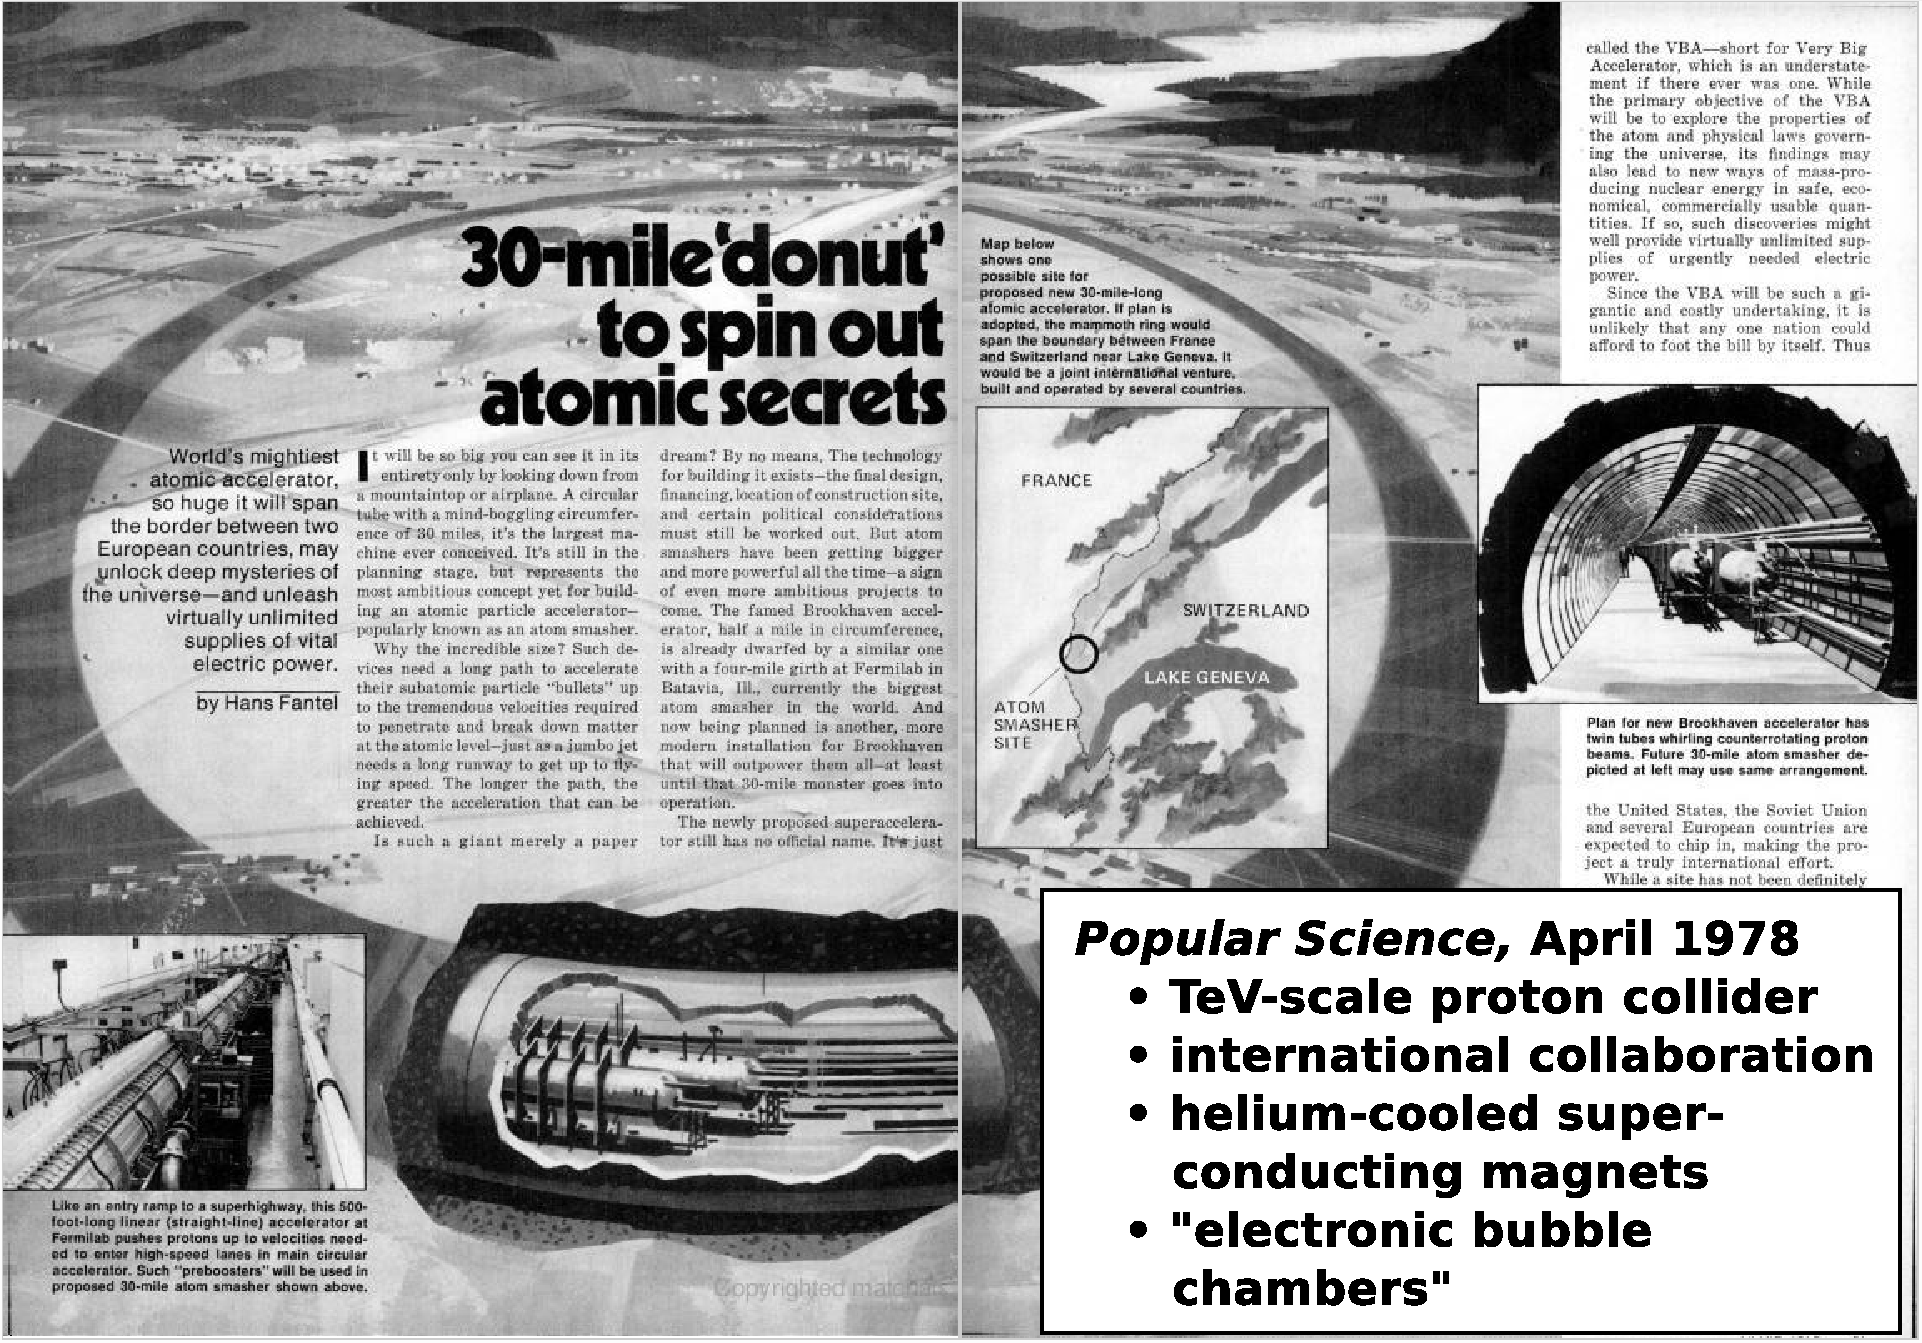
\includegraphics[width=\linewidth]{popular_mechanics.pdf}
\end{frame}

\begin{frame}
\frametitle{Introduction}
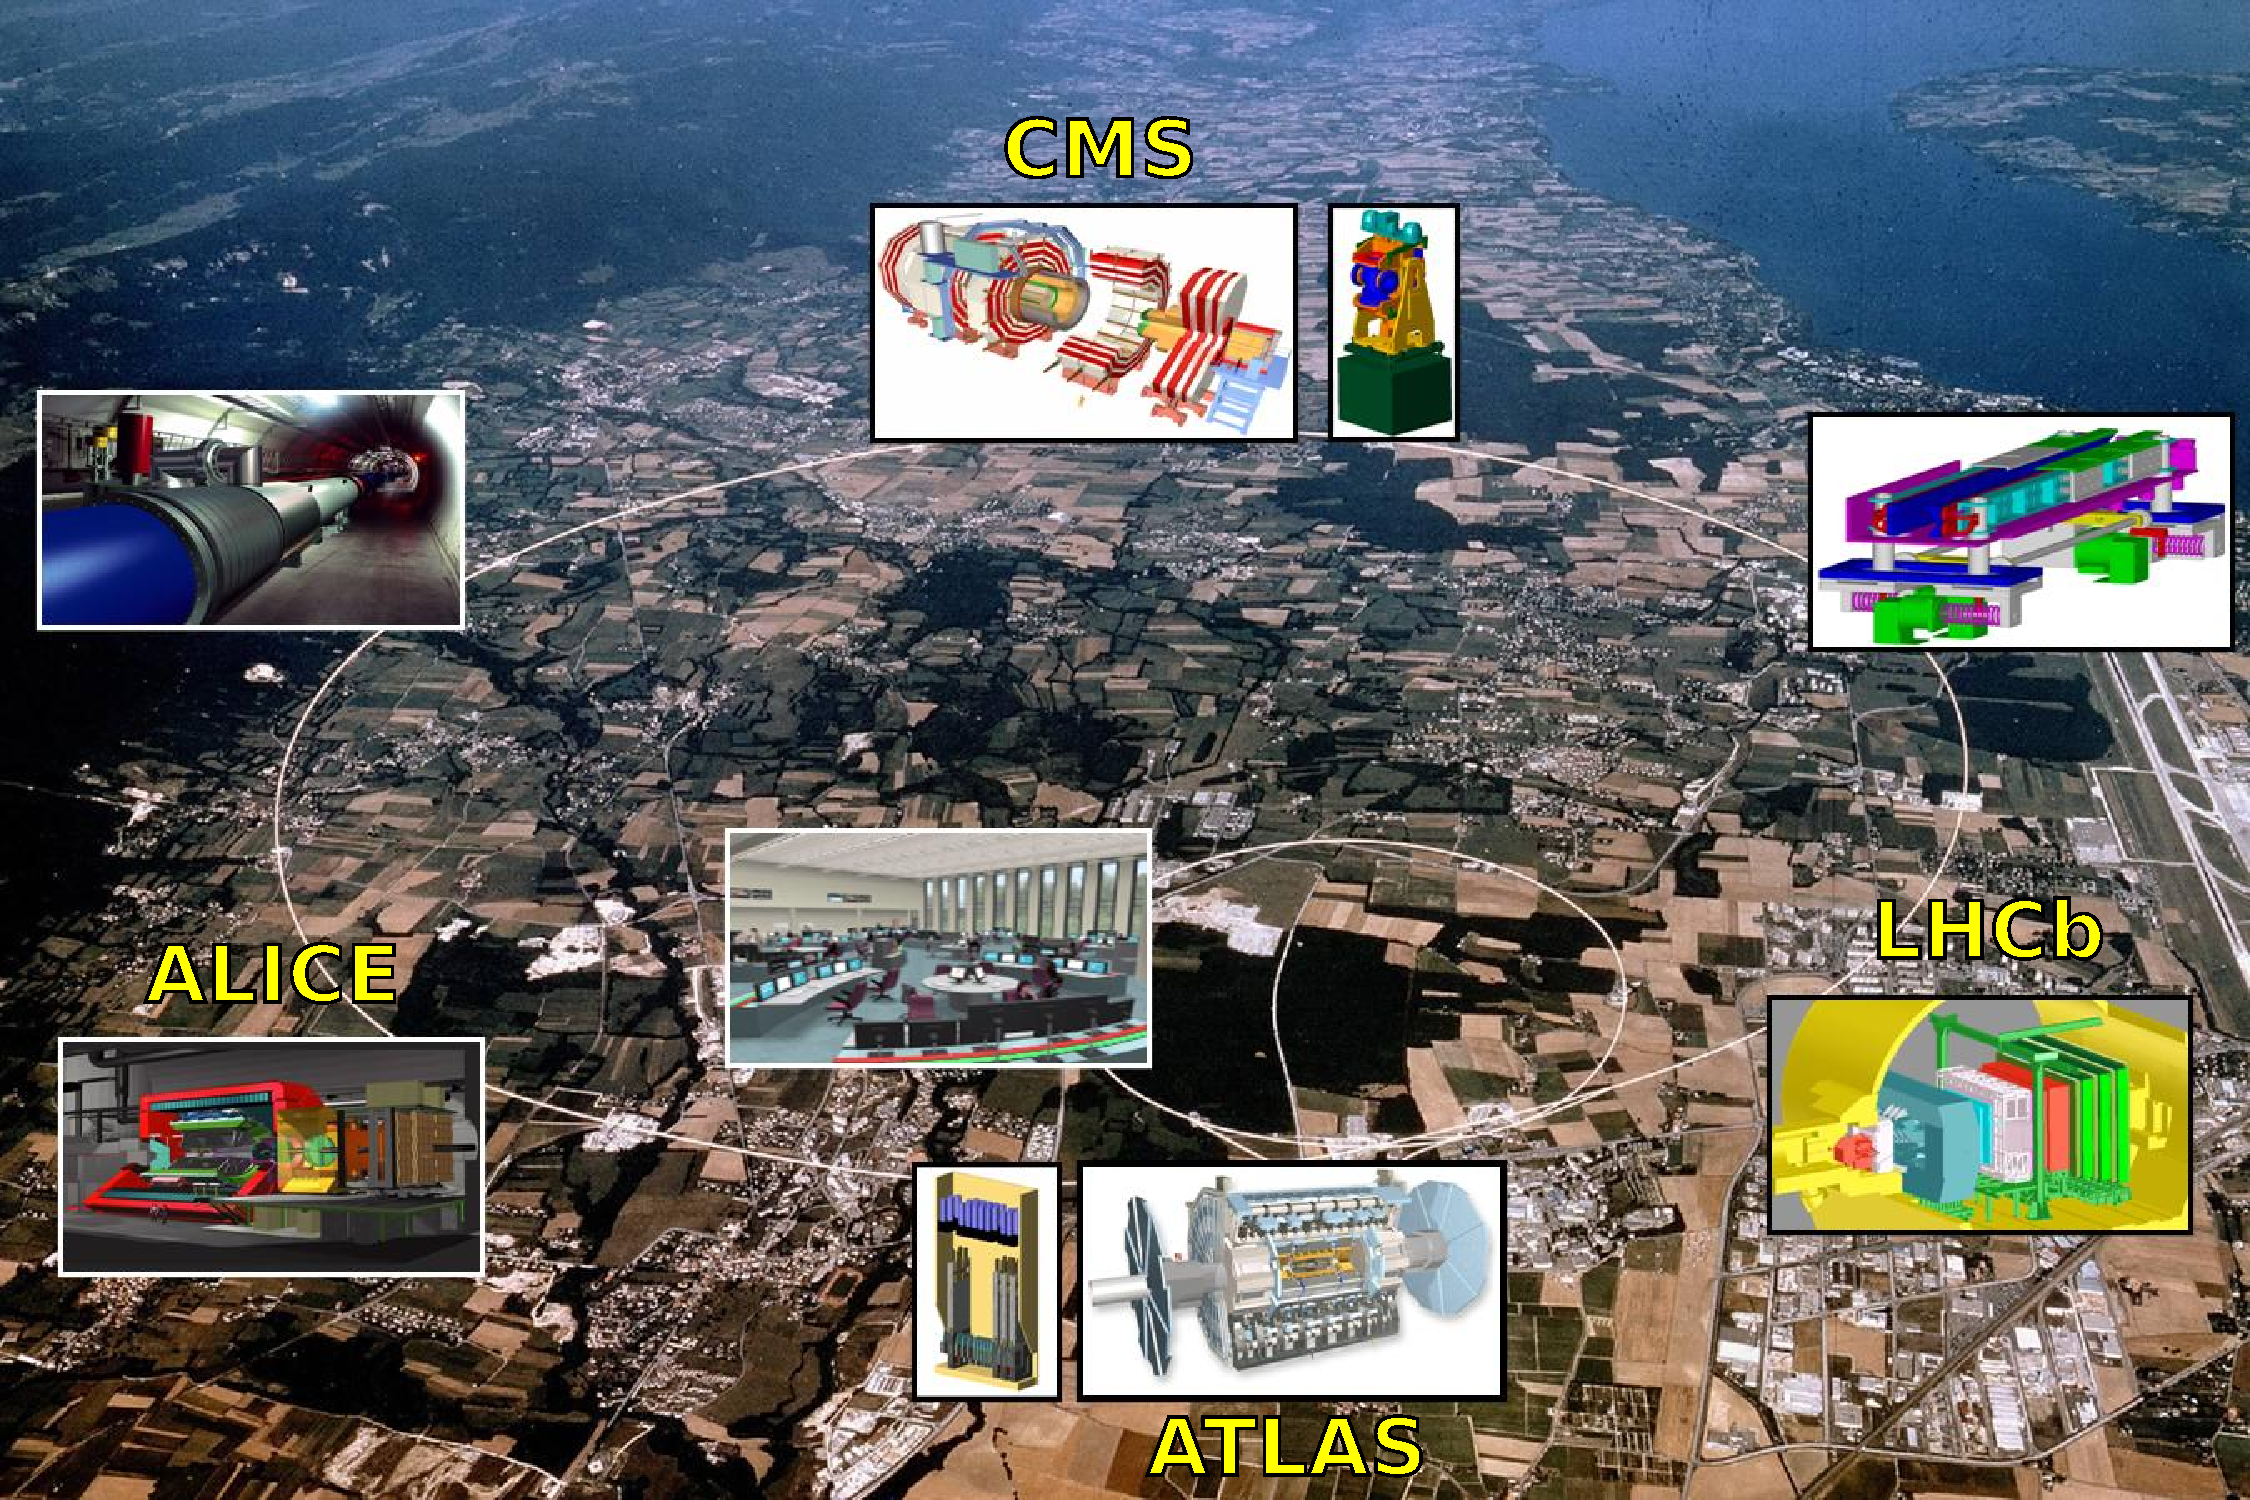
\includegraphics[width=\linewidth]{lhc.pdf}
\end{frame}

\begin{frame}
\frametitle{Introduction}
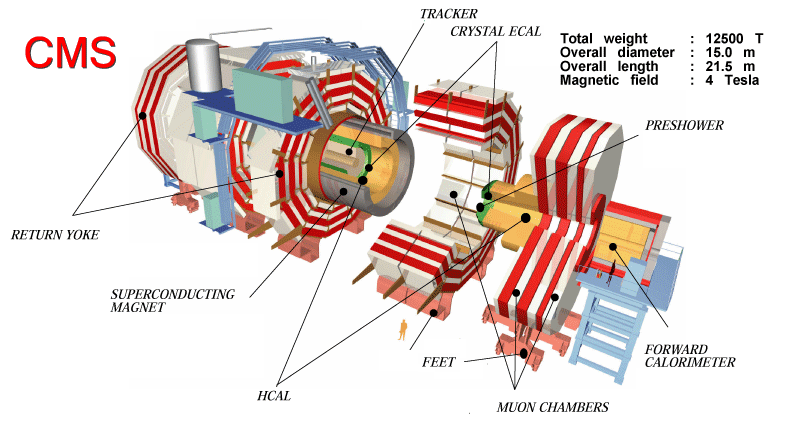
\includegraphics[height=3.3 cm]{cms_schematic.png}
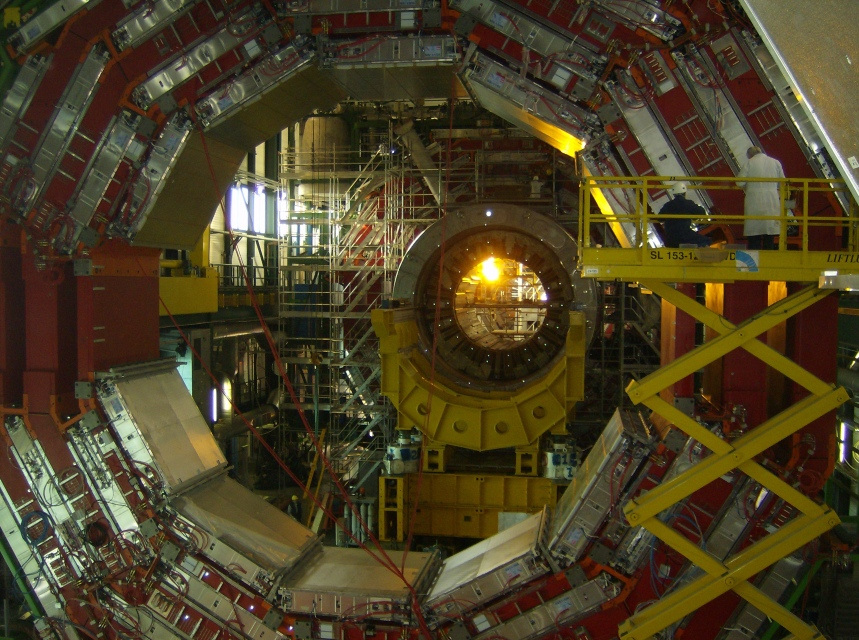
\includegraphics[height=3.3 cm]{sun_shines_in_the_detector.jpg}

\begin{itemize}
\item CMS is an all-purpose detector, designed for discovery

\item Modular for relatively easy access, strong
  $\vec{B}$-field, all-silicon tracker, all-software L2--L3 trigger

\item Approximate scale of the project: 66M pixel channels, 10M
  silicon channels, 75k crystals, 150k silicon preshower channels, 15k
  HCAL channels, 250 DT chambers (170k wires), 470 CSC chambers (200k
  wires), 900 RPC chambers, 50~kHz DAQ system (10k CPU cores), GRID
  computing (50k cores), 2M lines of offline source code\ldots
\end{itemize}
\end{frame}

\begin{frame}
\frametitle{Introduction}
\begin{columns}
\column{0.45\linewidth}
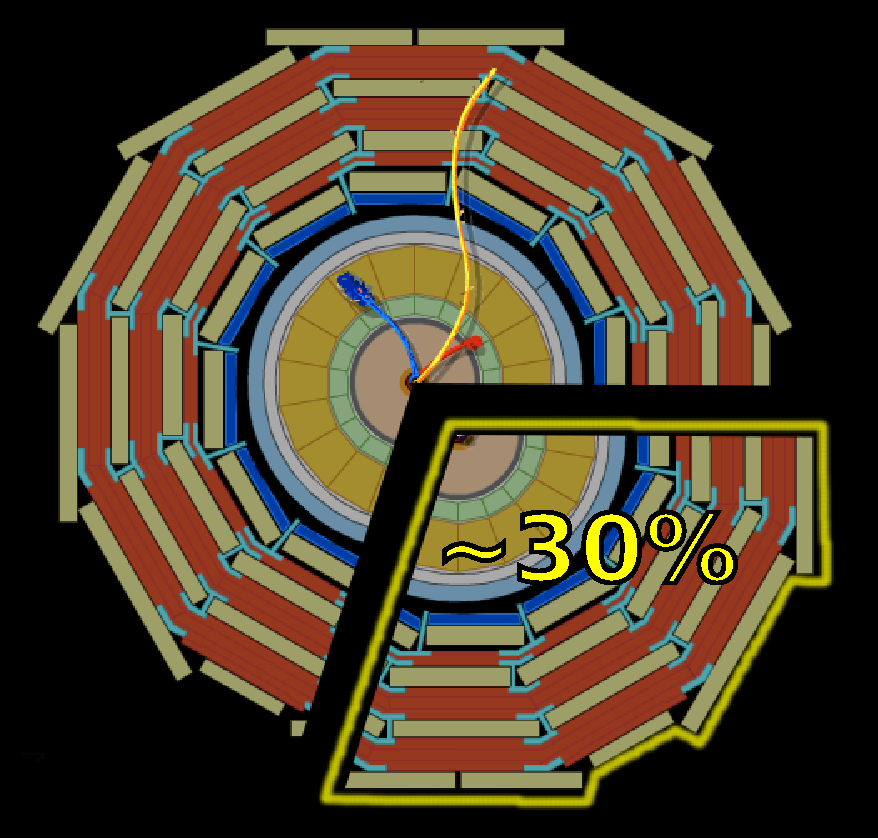
\includegraphics[width=\linewidth]{CMS_homepage.pdf}

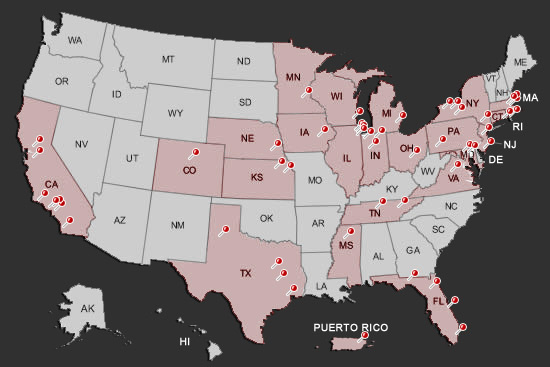
\includegraphics[width=\linewidth]{usa-map.jpg}
\column{0.55\linewidth}
\begin{itemize}
\item CMS: 190 institutions, 4700 participants, 1940 scientific
  authors, 800 students, 39 countries

\item US-CMS: 49 institutions, 1400 participants, 640 scientific
  authors, 200 graduate students

\item U.S.-led subsystems:

\vspace{-0.3 cm}
\begin{itemize}
\item hadron calorimeter
\item endcap muons
\item forward pixels
\item trigger
\end{itemize}

\item Strong U.S.\ participation:

\vspace{-0.3 cm}
\begin{itemize}
\item data acquisition
\item silicon strip tracker
\item electromagnetic calorimeter
\item computing
\item physics analyses
\end{itemize}
\end{itemize}
\end{columns}
\end{frame}

\begin{frame}
\frametitle{Outline for this talk}

\textcolor{darkblue}{\normalsize By October 2009, the conventional wisdom
  of what to expect in the first year of LHC physics went something
  like the following:}

\begin{itemize}\setlength{\itemsep}{0.3 cm}
\item<1-> ``Expect a rapid rise in luminosity at the beginning\ldots''

\item<2-> ``The first physics measurements will be dedicated to
  rediscovering the Standard Model\ldots''

\item<3-> ``Beyond the Standard Model will be exotica searches,
  extending di-object mass limits, then SUSY and Higgs\ldots''

\item<4-> ``Expect the unexpected: we'll probably find things we
  weren't even looking for\ldots''

\item<5-> ``Don't expect everything to work at first\ldots''
\begin{itemize}
\item here, we were surprised: even complex techniques like
  $b$-tagging, missing energy, particle flow, etc., {\it do} seem to
  be working as expected from simulations
\end{itemize}
\end{itemize}
\end{frame}

%% \begin{frame}
%% \frametitle{Introduction}
%% \begin{itemize}\setlength{\itemsep}{0.75 cm}
%% \item 
%% \end{itemize}
%% %% \hspace{-0.83 cm} \textcolor{darkblue}{\Large Outline2}
%% \end{frame}

\section*{Rapid rise in luminosity}
\begin{frame}
\begin{center}
\Huge \textcolor{blue}{Rapid rise in luminosity \\ and data collection}
\end{center}
\end{frame}

\begin{frame}
\frametitle{Luminosity and data collection}

\begin{columns}
\column{0.5\linewidth}
\begin{center}
Integrated luminosity: linear scale

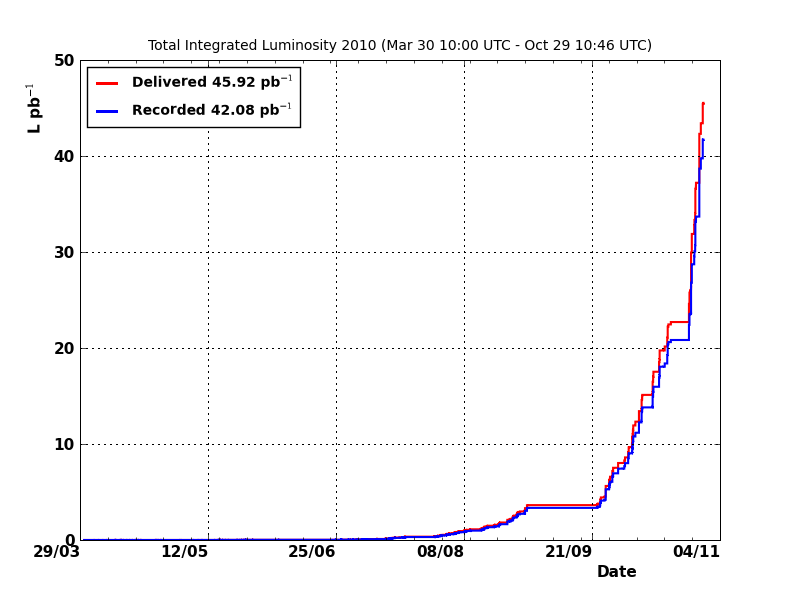
\includegraphics[width=\linewidth]{totallumivstime_3.png}
\end{center}

\column{0.5\linewidth}
\begin{center}
Integrated luminosity: log scale

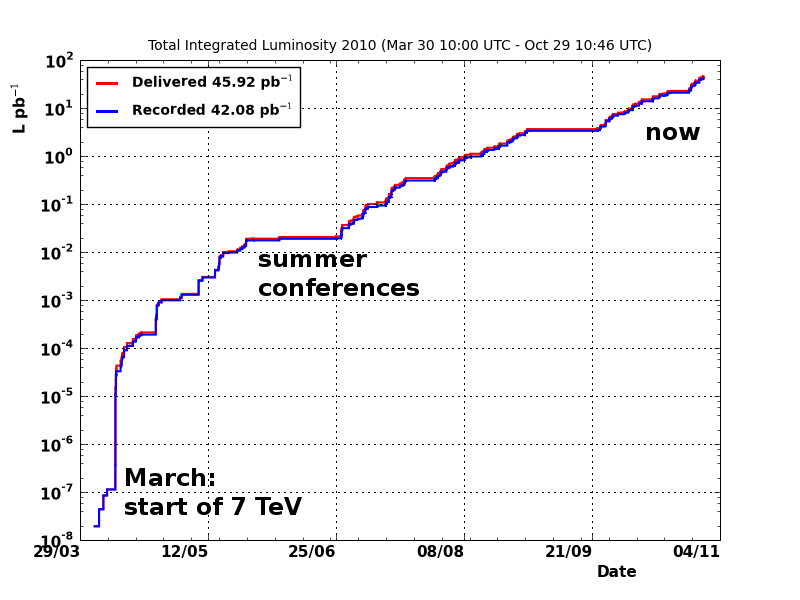
\includegraphics[width=\linewidth]{totallumivstime_log_3.png}
\end{center}
\end{columns}

\begin{columns}
\column{0.5\linewidth}
\begin{itemize}
\item Steps in luminosity from $\mathcal{L} = 10^{27}$ to
  $10^{32}$~Hz/cm$^2$
\item Not unusual for a weekend to double the entire dataset
\item Maintaining $\sim$90\% livetime (requiring all subsystems)
\end{itemize}

\column{0.5\linewidth}
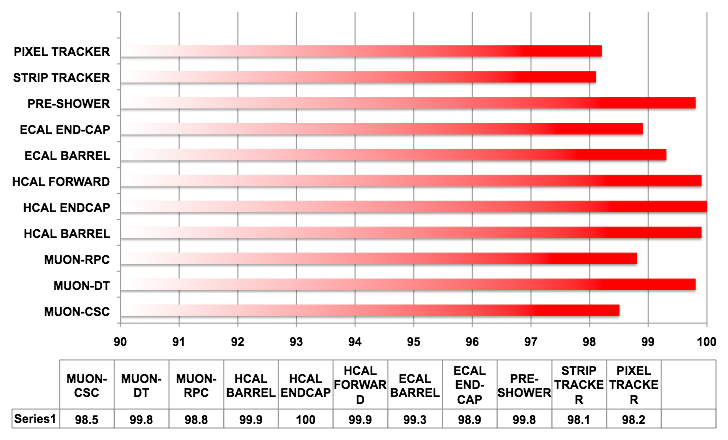
\includegraphics[width=\linewidth]{livetime.png}
\end{columns}
\end{frame}

\begin{frame}
\frametitle{Luminosity and data collection}

\begin{itemize}
\item We want wide-open triggers at first, narrowing as \mbox{luminosity increases\hspace{-1 cm}}

\item To minimize prescaling of good physics, we need accurate predictions of cross-sections, despite the fact that Monte Carlos have not been tuned to 7~TeV $pp$ yet

\item Bootstrap trigger estimates on previous datasets
\end{itemize}

\vspace{-0.3 cm}
\begin{columns}
\column{0.6\linewidth}
\begin{center}
Predicting trigger rates from MC and verifying with early data:

\vspace{0.4 cm}
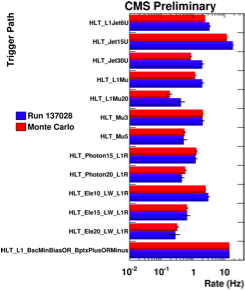
\includegraphics[height=2.8 cm]{trigger1.png}
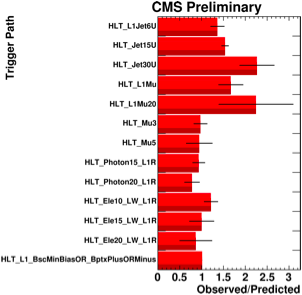
\includegraphics[height=2.8 cm]{trigger2.png}
\end{center}
\column{0.6\linewidth}
\begin{center}
Predicting rates from early data extrapolated to higher luminosities:

\vspace{0.4 cm}
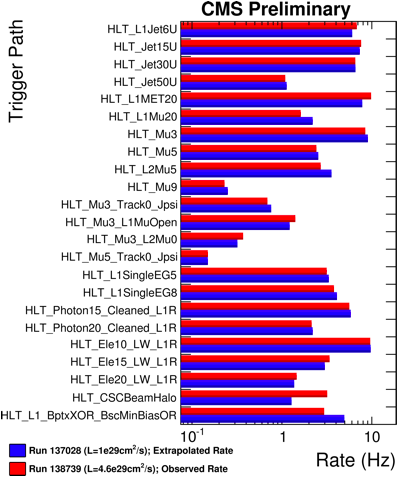
\includegraphics[height=2.8 cm]{trigger3.png}
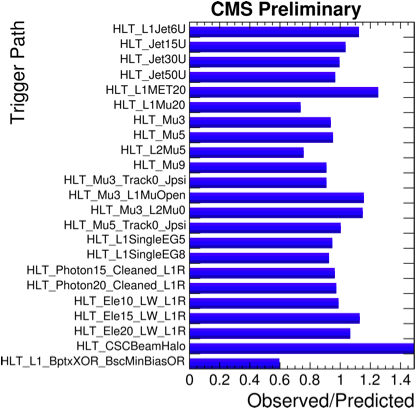
\includegraphics[height=2.8 cm]{trigger4.png}
\end{center}
\end{columns}

%% \begin{itemize}
%% \item Trigger synchronization refined in zero-bias timing scans:
%% \end{itemize}
%% \begin{center}
%% 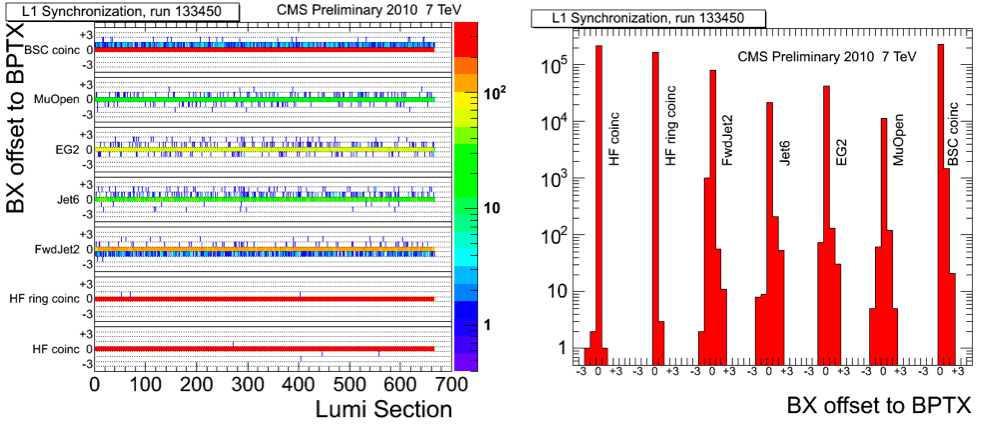
\includegraphics[width=0.6\linewidth]{triggersynch.png}
%% \end{center}
\end{frame}

\begin{frame}
\frametitle{Luminosity and data collection}
\begin{columns}
\column{0.5\linewidth}
\mbox{\hspace{0.5 cm}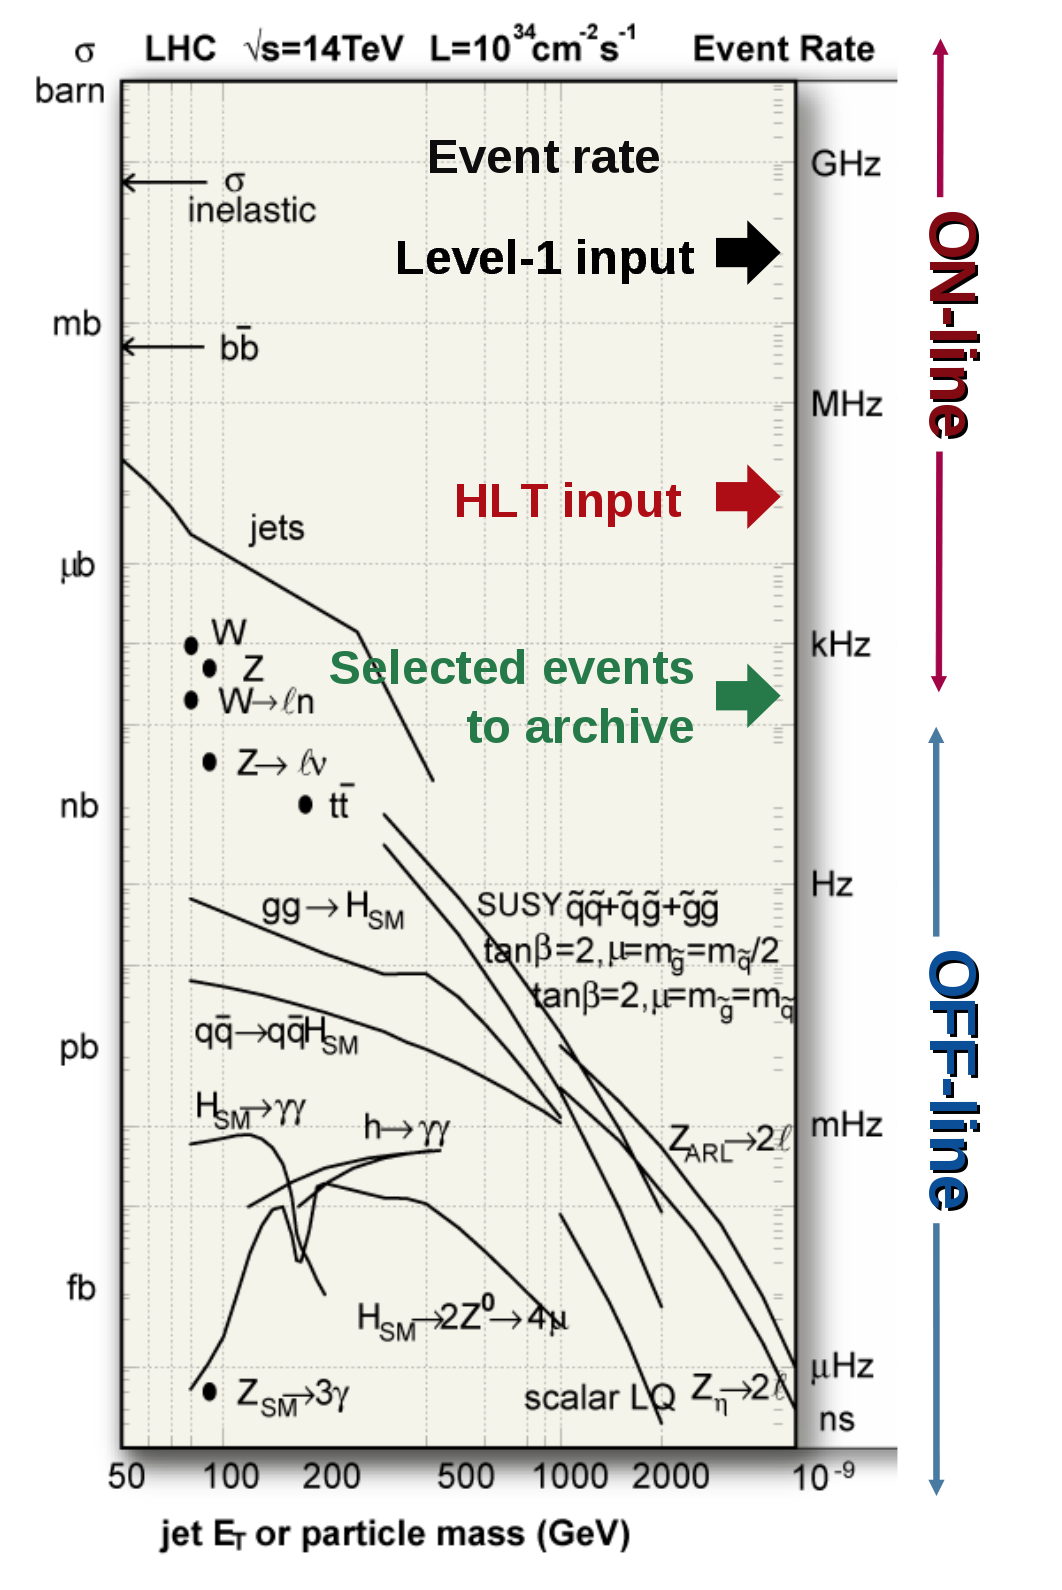
\includegraphics[width=\linewidth]{triggerrates.png}}
\column{0.6\linewidth}
\begin{itemize}
\item L1 trigger: 45--70~kHz
\item HLT (data-logging): \mbox{350--600~Hz\hspace{-1 cm}}
\item Sample turn-on curves from data:

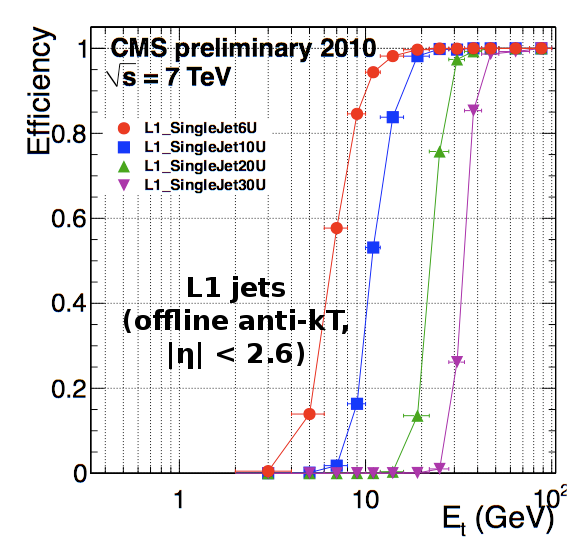
\includegraphics[width=0.5\linewidth]{turnon_jets.png}
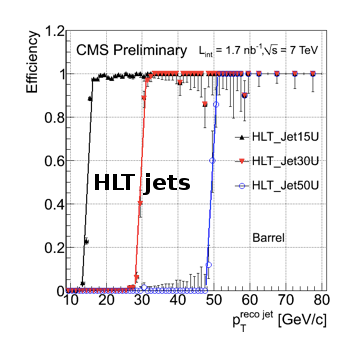
\includegraphics[width=0.5\linewidth]{turnon_hltjets.png}

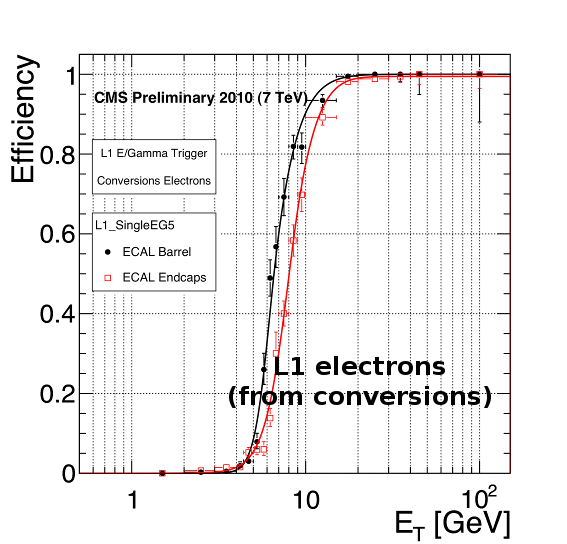
\includegraphics[width=0.5\linewidth]{turnon_electrons.png}
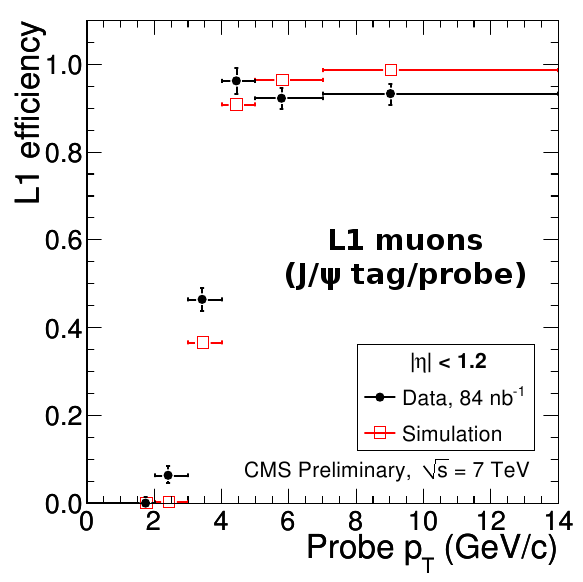
\includegraphics[width=0.5\linewidth]{turnon_muons.png}
\end{itemize}
\end{columns}
\end{frame}

\section*{Rediscovering the Standard Model}
\begin{frame}
\begin{center}
\Huge \textcolor{blue}{Rediscovering \\ the Standard Model}
\end{center}
\end{frame}

\begin{frame}
\frametitle{Rediscovering the Standard Model}
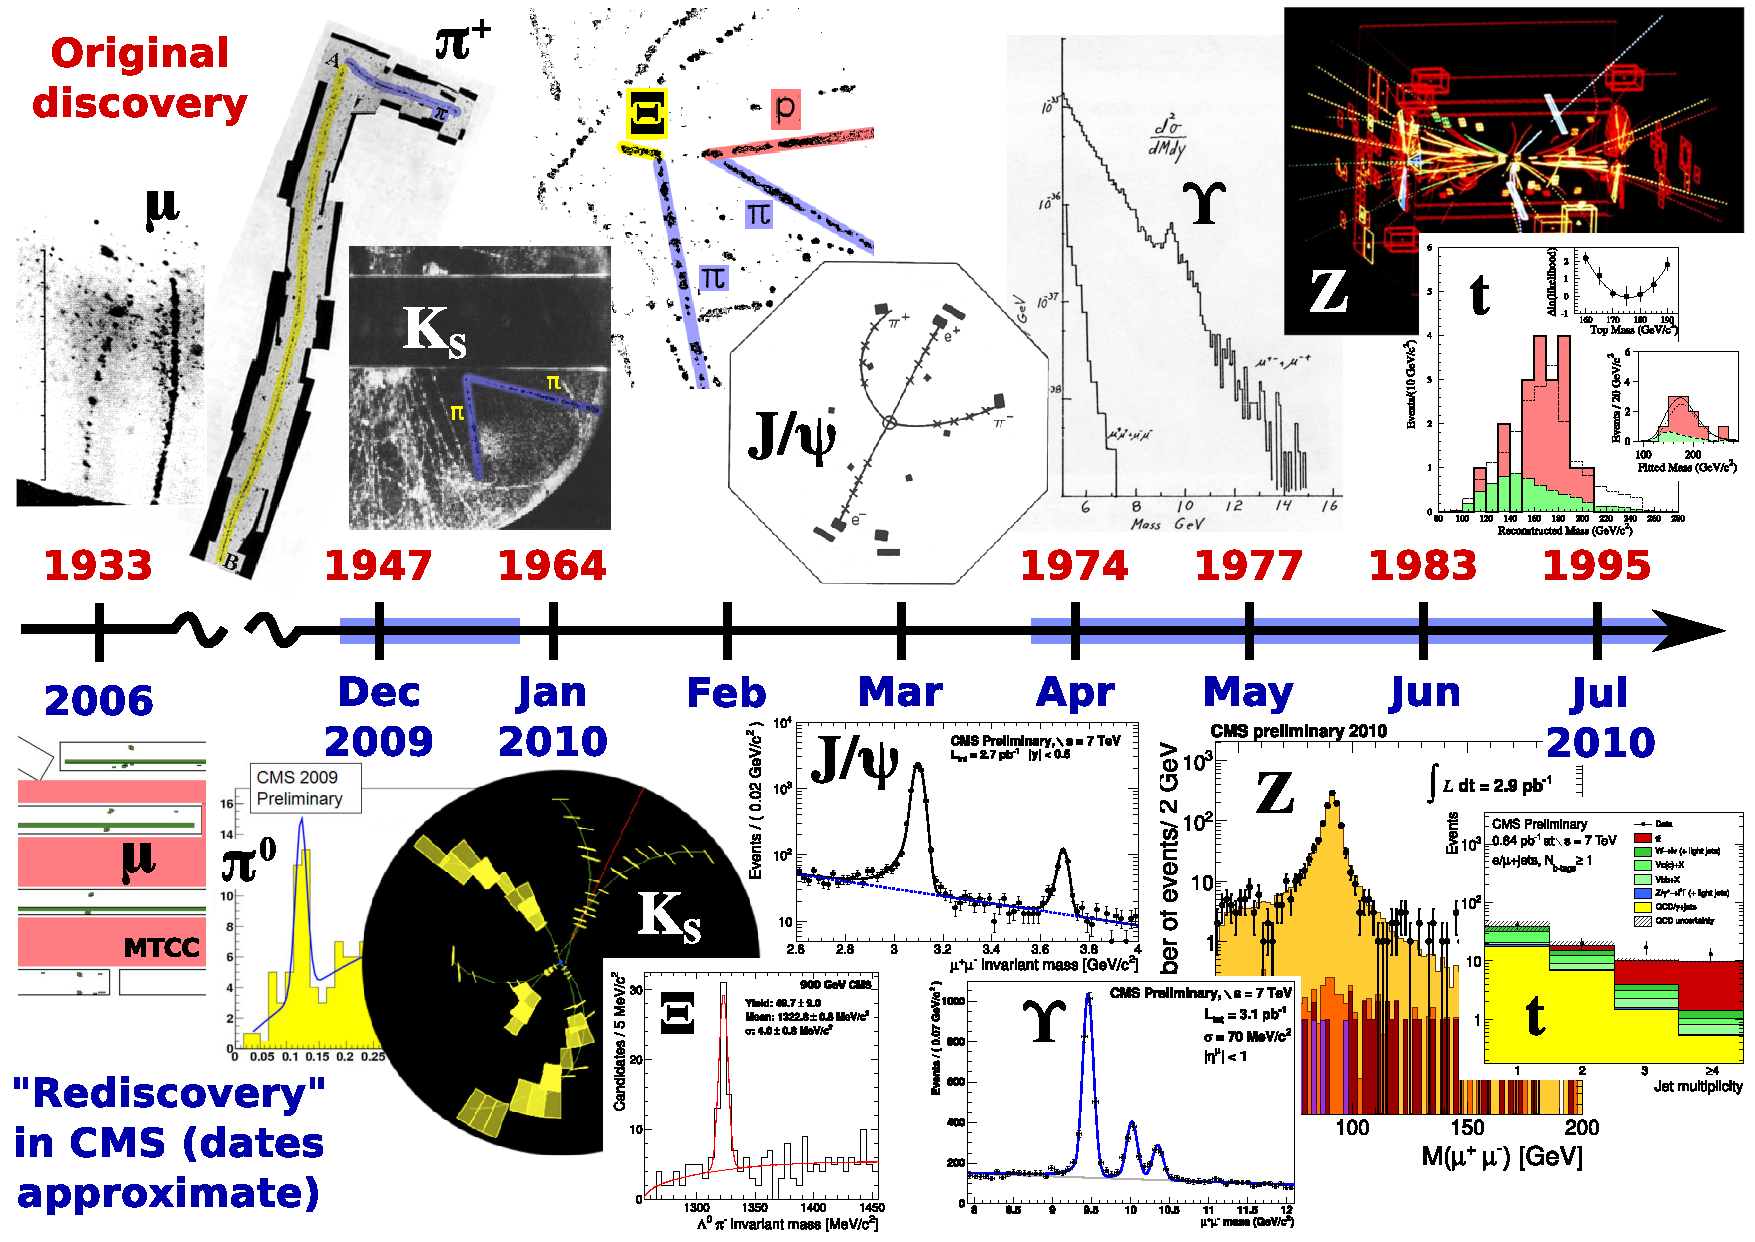
\includegraphics[width=\linewidth]{timeline.pdf}
\end{frame}

\begin{frame}
\frametitle{Rediscovering the Standard Model}
\framesubtitle{Sample plots}

\vspace{-0.5 cm}
\begin{itemize}
\item The whole self-adjoint vector resonance spectrum:
\end{itemize}

\vspace{-0.6 cm}
\begin{columns}
\column{0.5\linewidth}
\begin{center} $e^+e^-$ log mass \end{center}

\vspace{-0.3 cm}
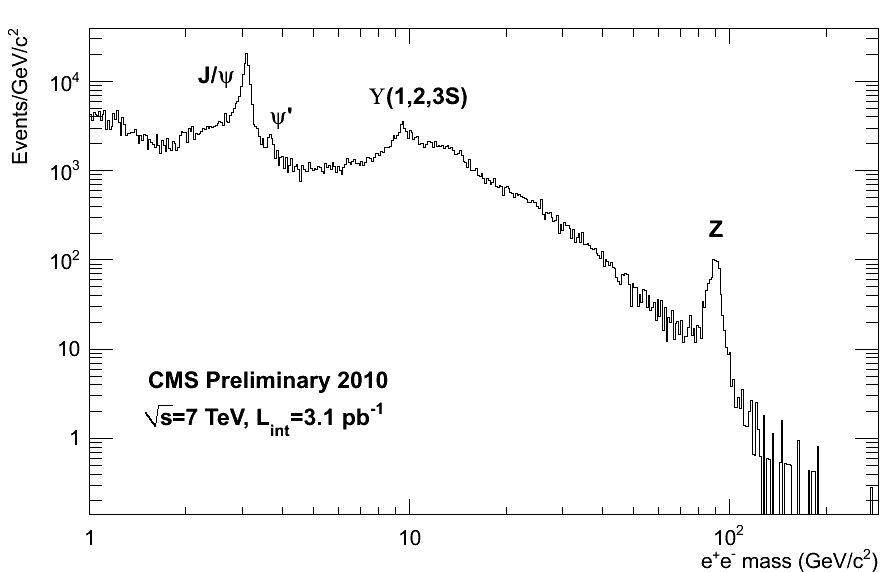
\includegraphics[width=\linewidth]{spectrum_ee.png}

\column{0.5\linewidth}
\begin{center} $\mu^+\mu^-$ log mass \end{center}

\vspace{-0.3 cm}
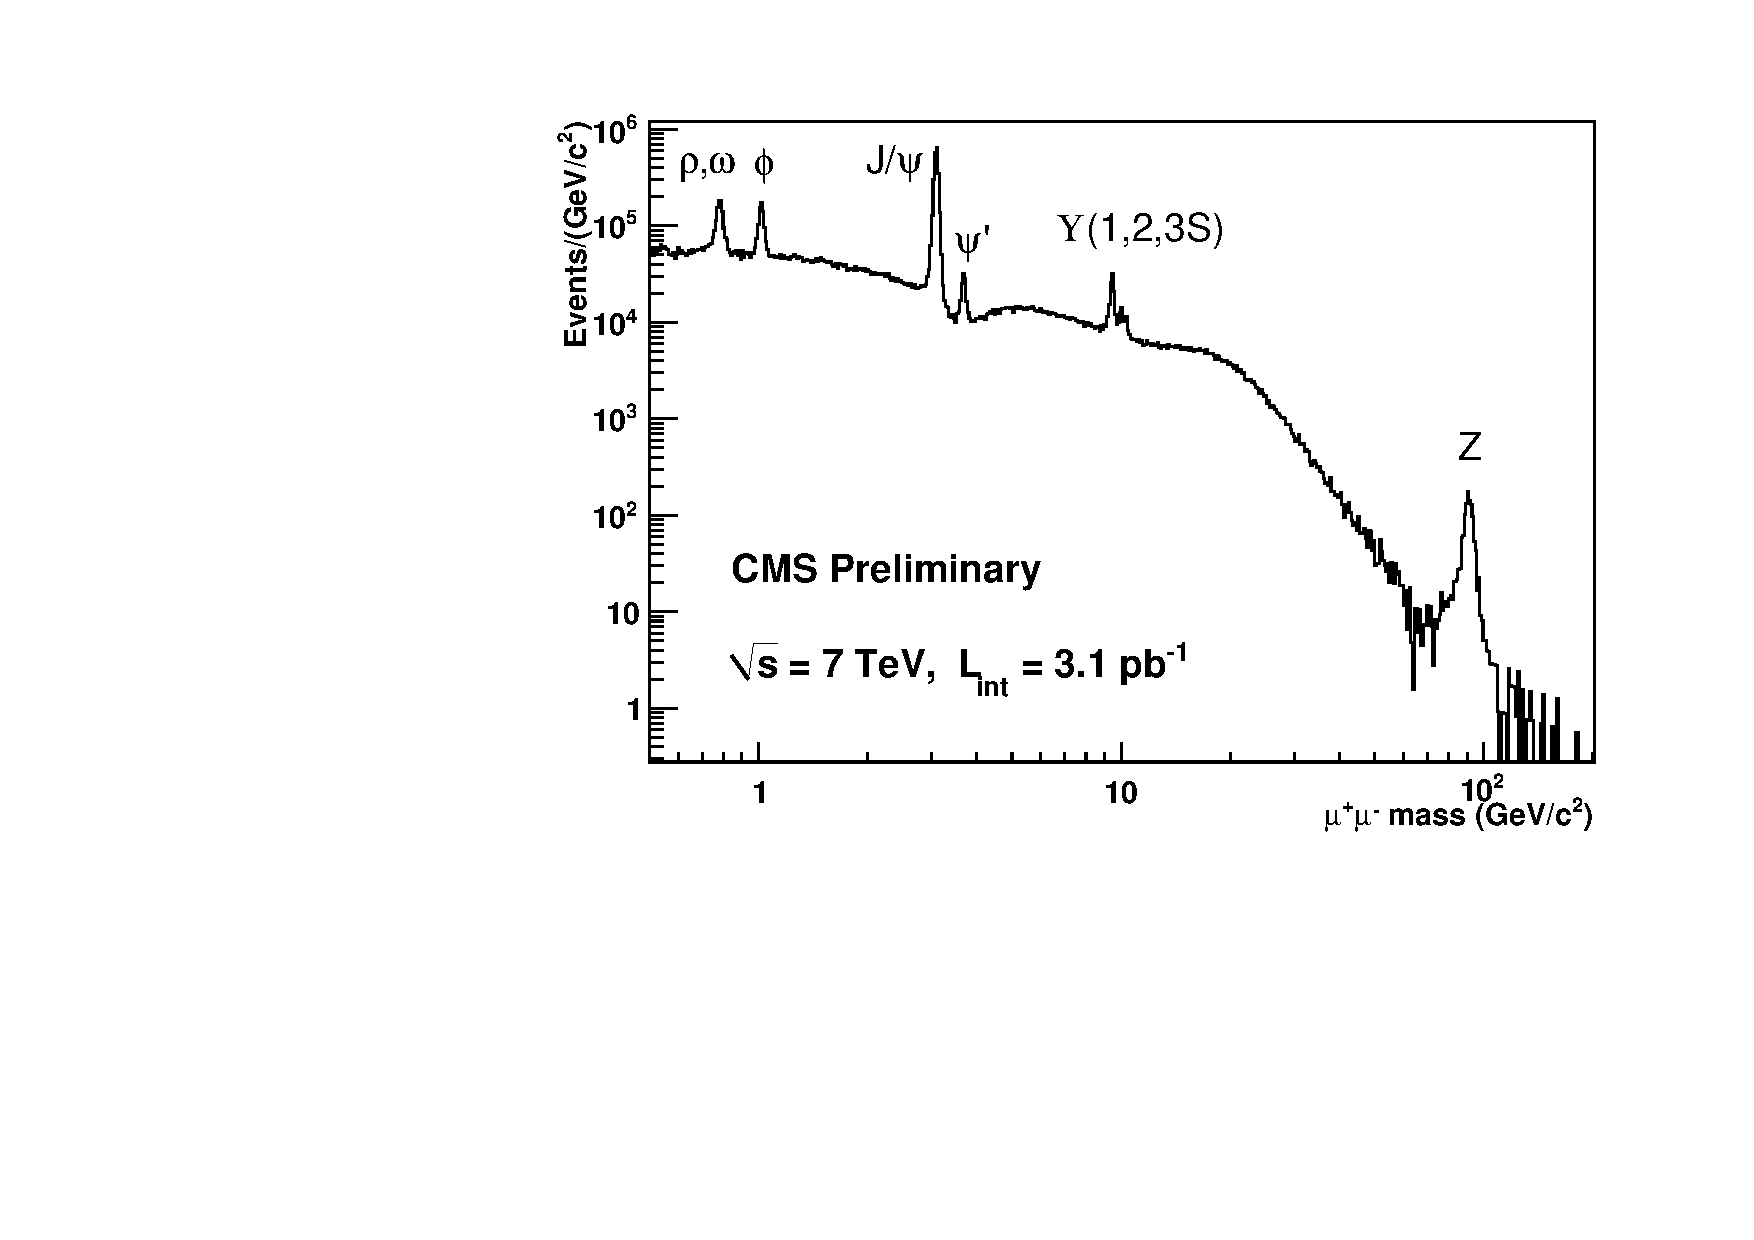
\includegraphics[width=\linewidth]{spectrum_mumu.pdf}
\end{columns}

\begin{itemize}
\item And a few other nice examples:
\end{itemize}

\vspace{-0.1 cm}
\mbox{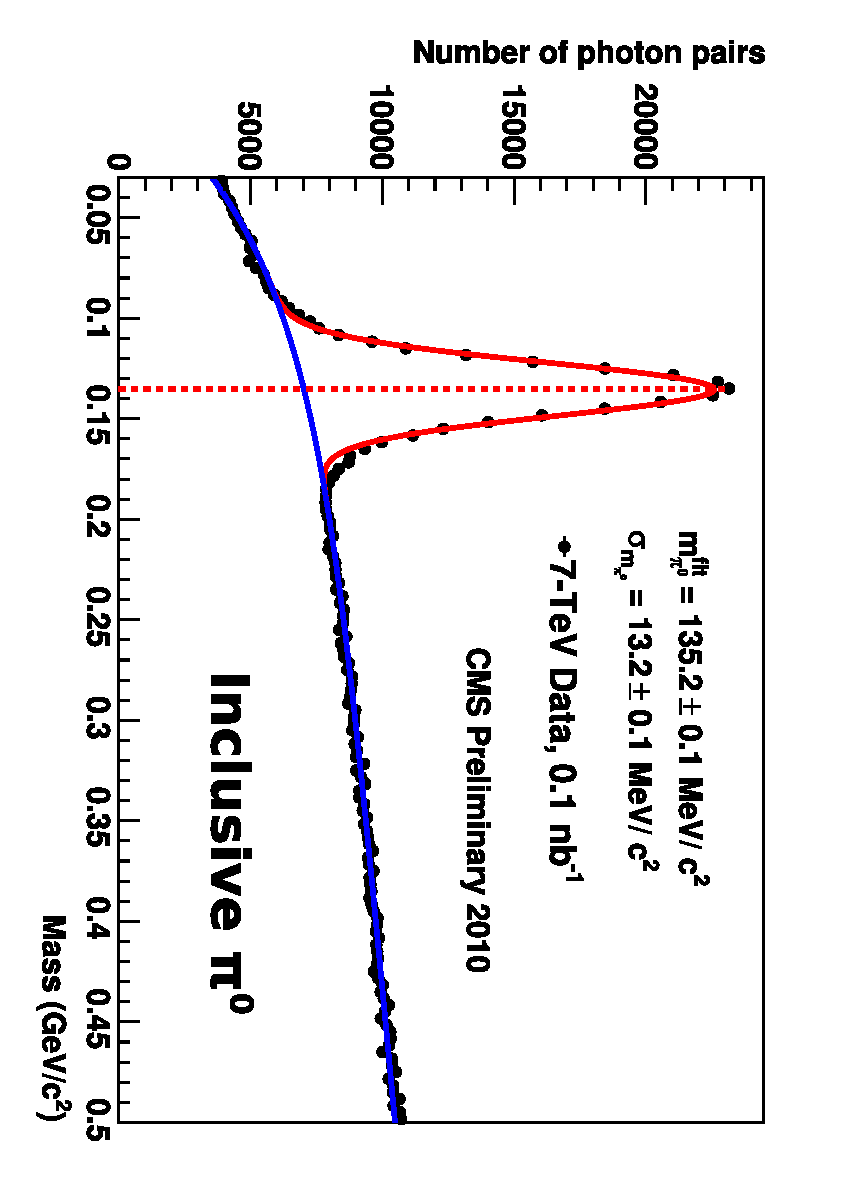
\includegraphics[width=2.3 cm, angle=90]{pi0_now.pdf}\hspace{0.1 cm}
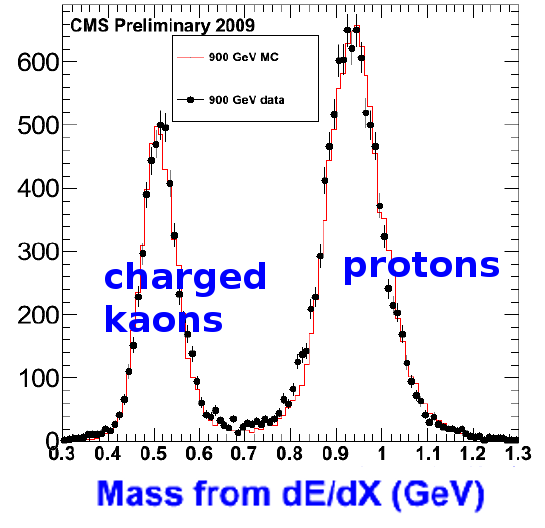
\includegraphics[height=2.3 cm]{mass_from_dedx.png}\hspace{0.1 cm}
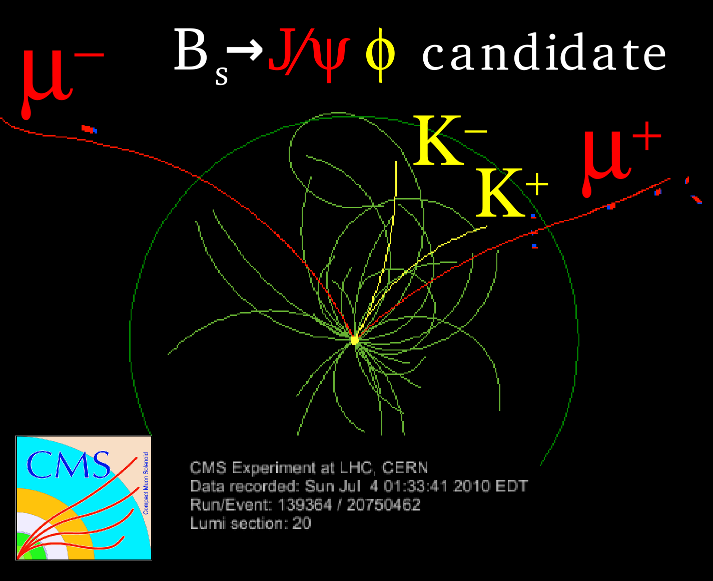
\includegraphics[height=2.1 cm]{BstoJpsiPhi.png}\hspace{0.1 cm}
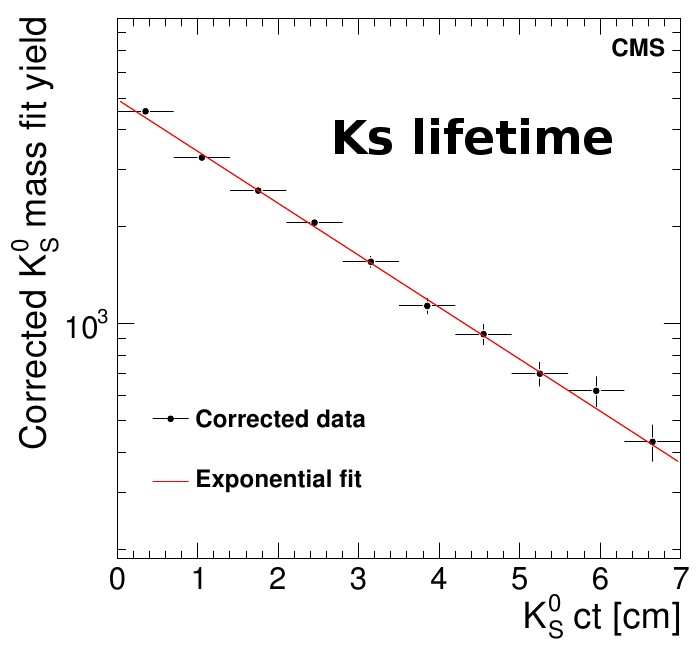
\includegraphics[height=2.3 cm]{K0S_lifetime.png}\hspace{-1 cm}}
\end{frame}

\begin{frame}
\frametitle{Rediscovering the Standard Model}
\framesubtitle{Electroweak bosons}
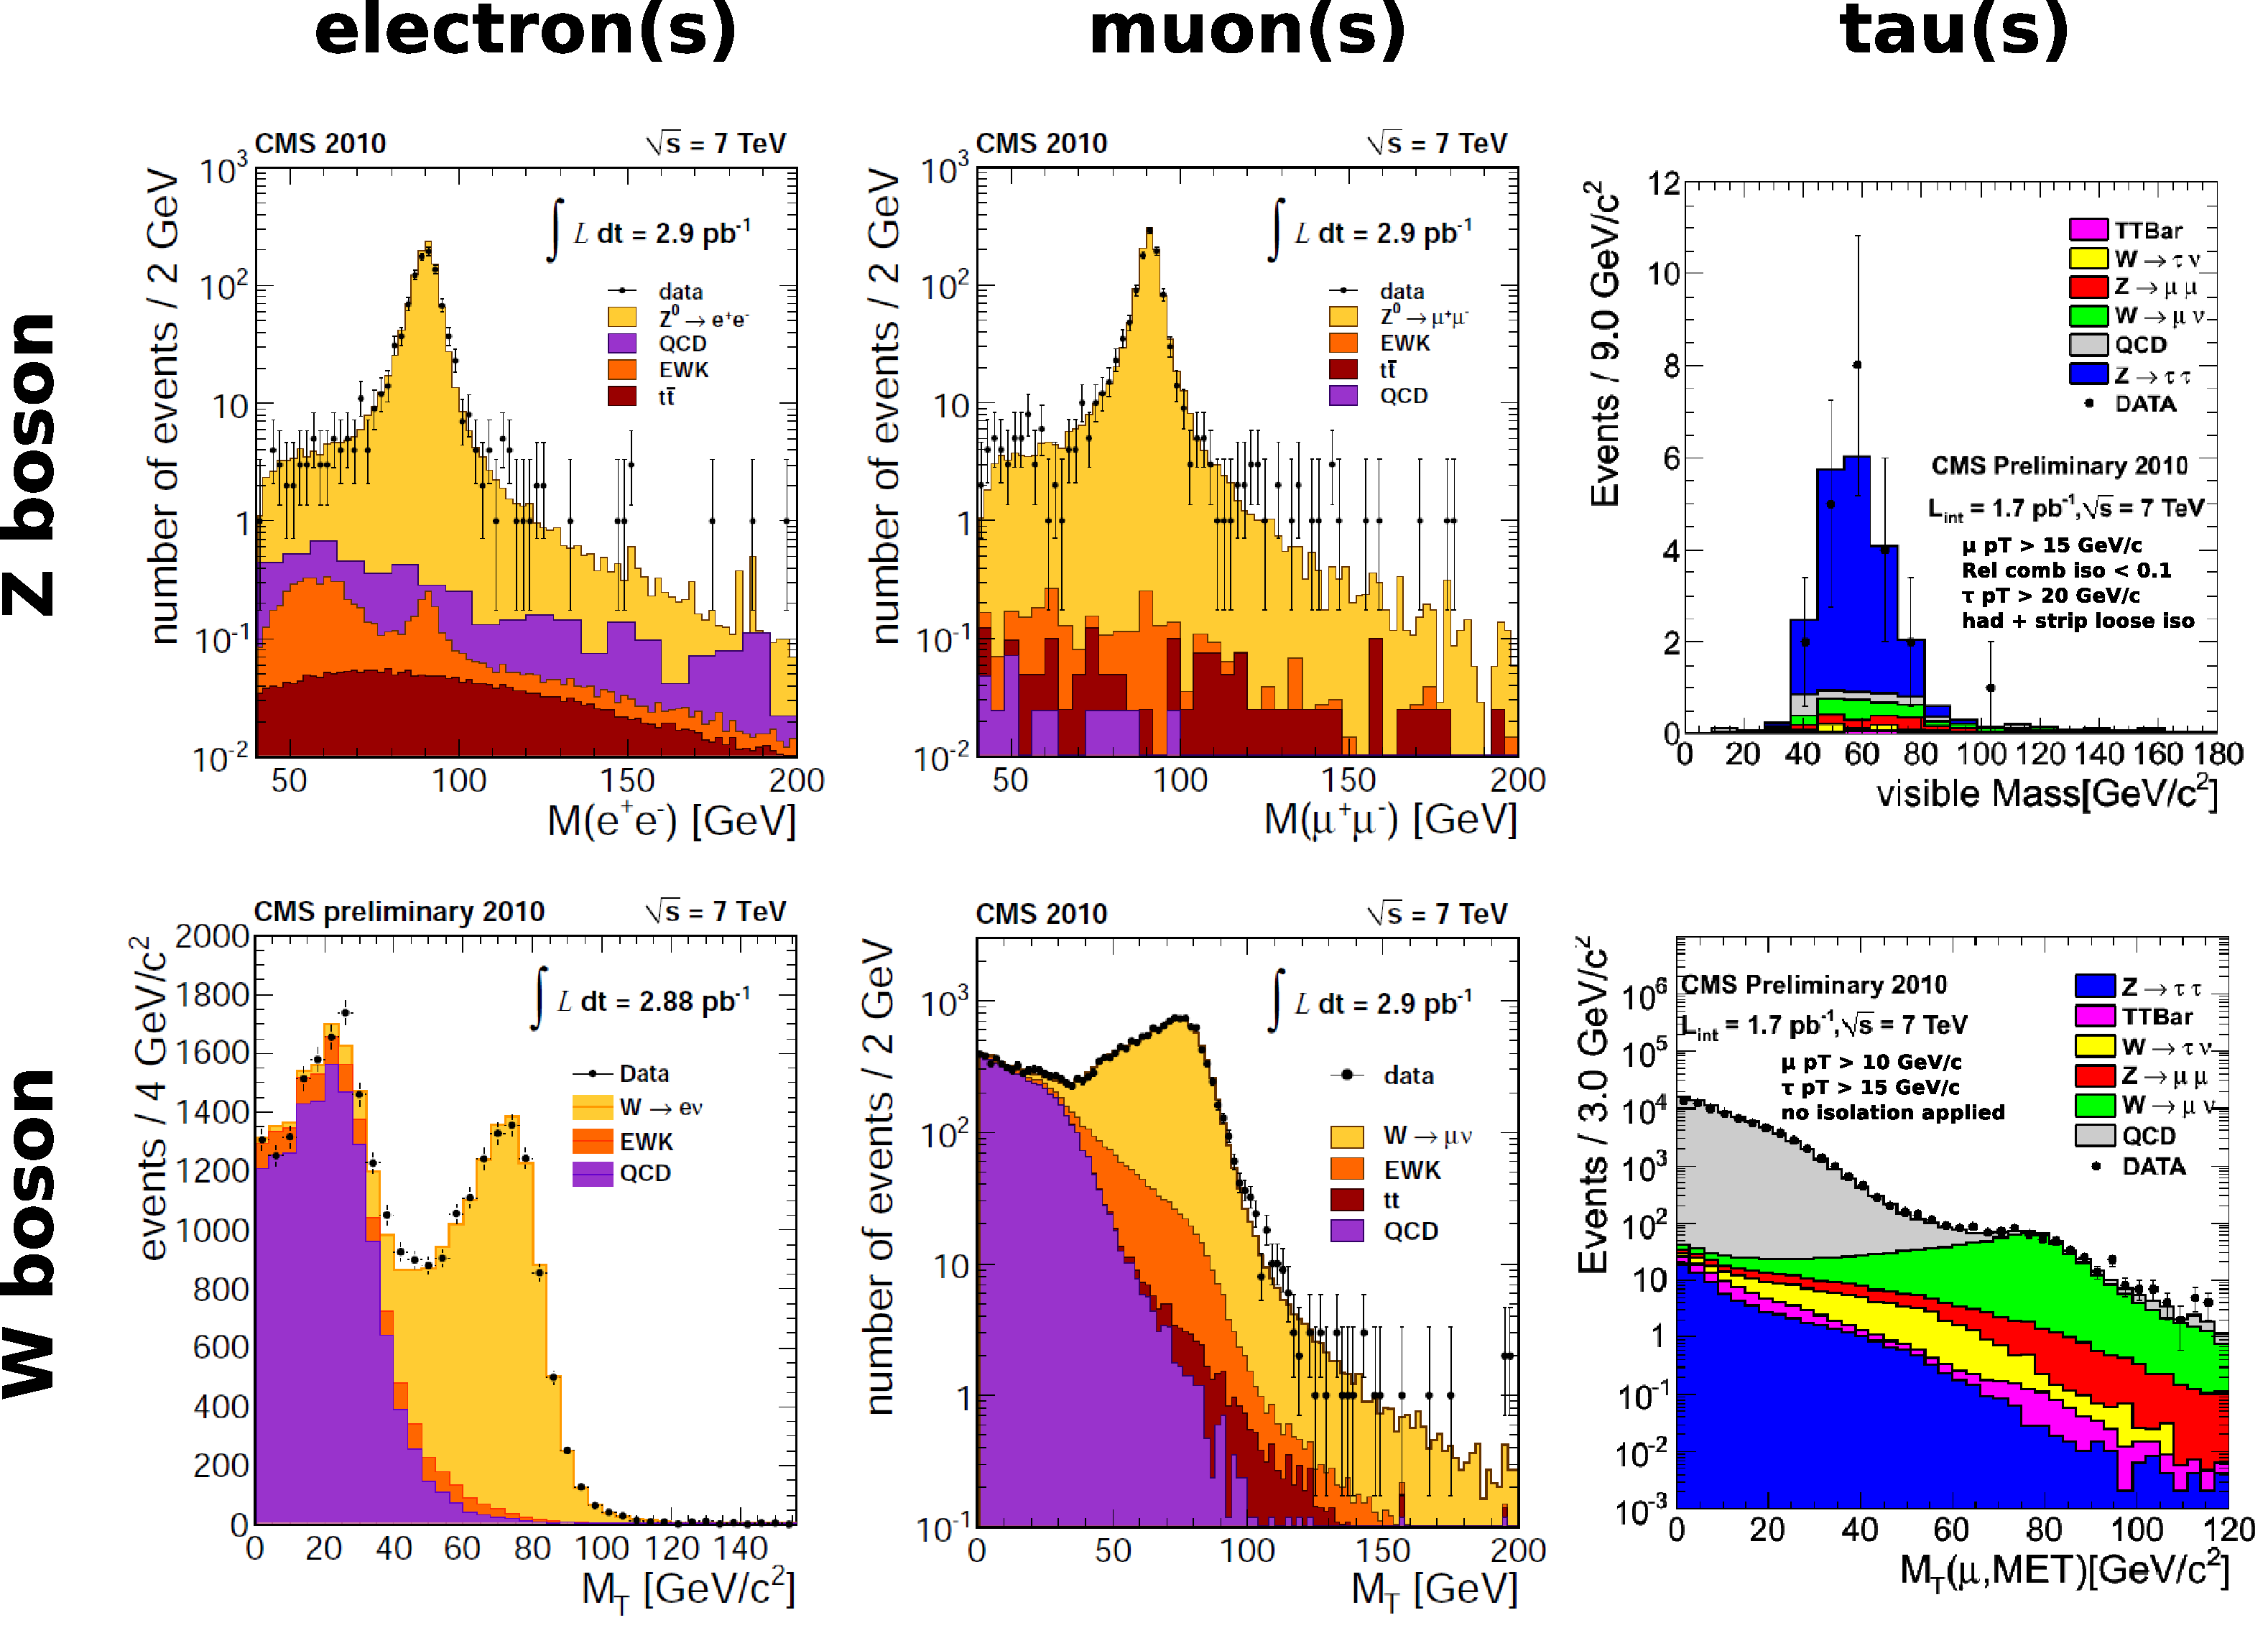
\includegraphics[width=\linewidth]{electroweak.pdf}
\end{frame}

\begin{frame}
\frametitle{Rediscovering the Standard Model}
\framesubtitle{Electroweak bosons}
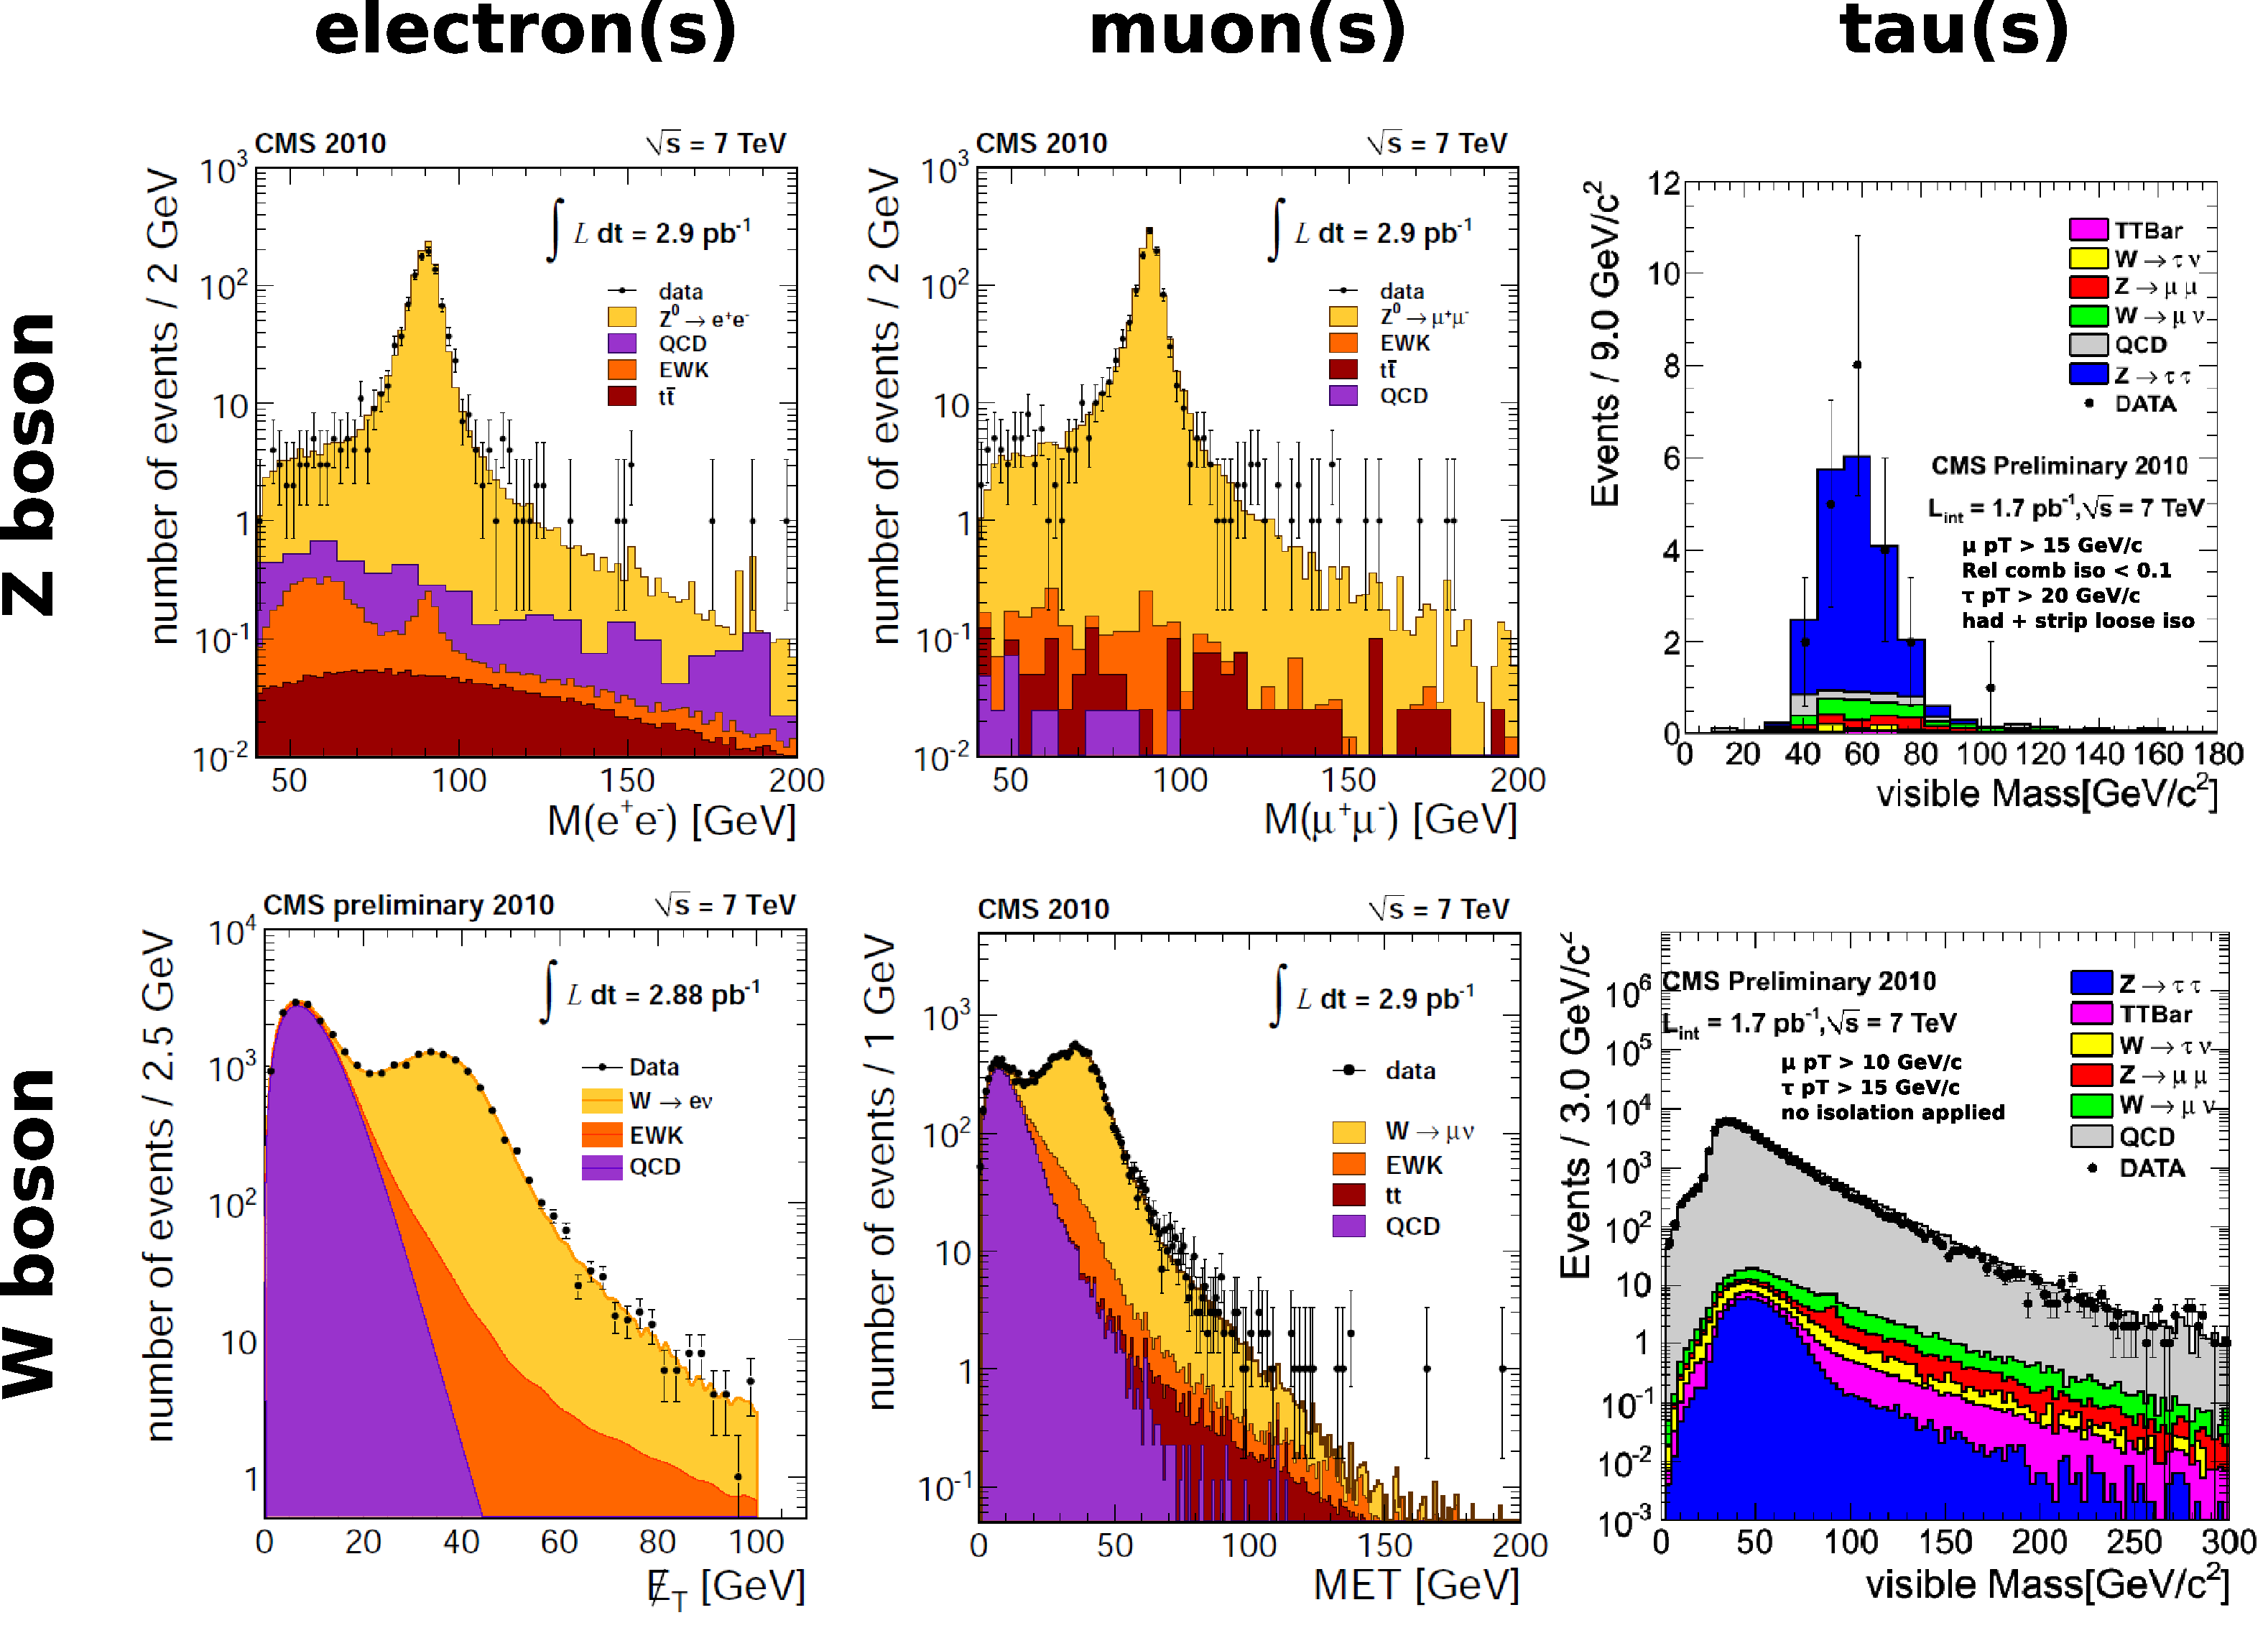
\includegraphics[width=\linewidth]{electroweak2.pdf}
\end{frame}

\begin{frame}
\frametitle{Rediscovering the Standard Model}
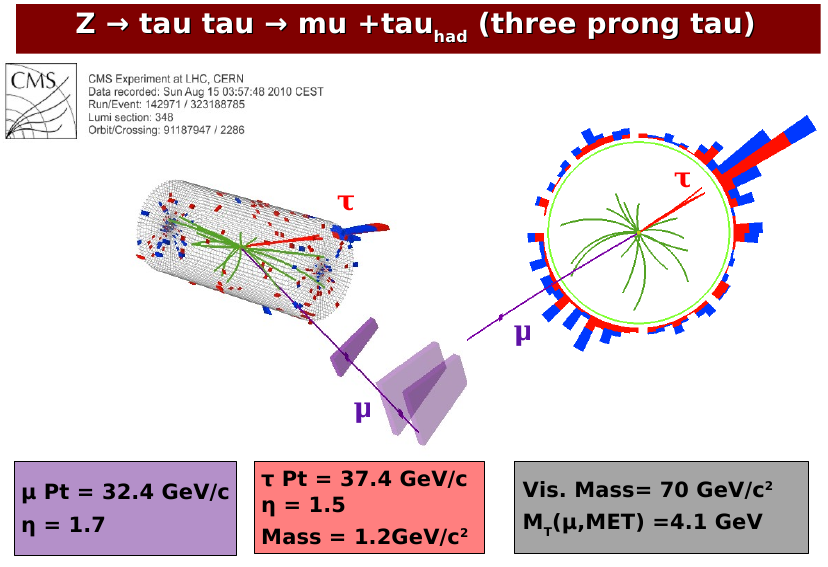
\includegraphics[width=\linewidth]{Ztautau_display.png}
\end{frame}

\begin{frame}
\frametitle{Rediscovering the Standard Model}
\framesubtitle{Electroweak physics results}
\begin{columns}
\column{0.4\linewidth}
\begin{center}
\textcolor{darkblue}{Production cross-sections}

(see Andrew Kubik's talk)

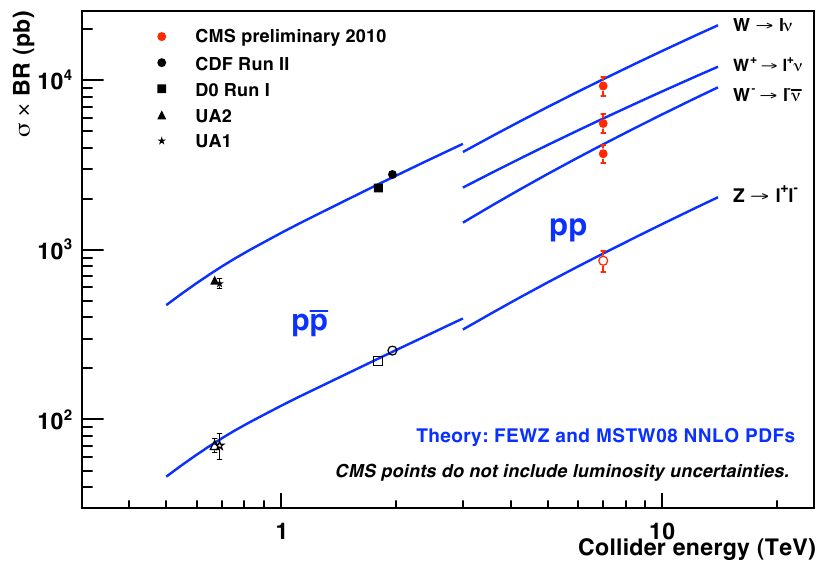
\includegraphics[width=\linewidth]{electroweak_crosssections.png}

\vspace{0.2 cm}
\textcolor{darkblue}{$W^\pm$ charge asymmetry}

\hfill 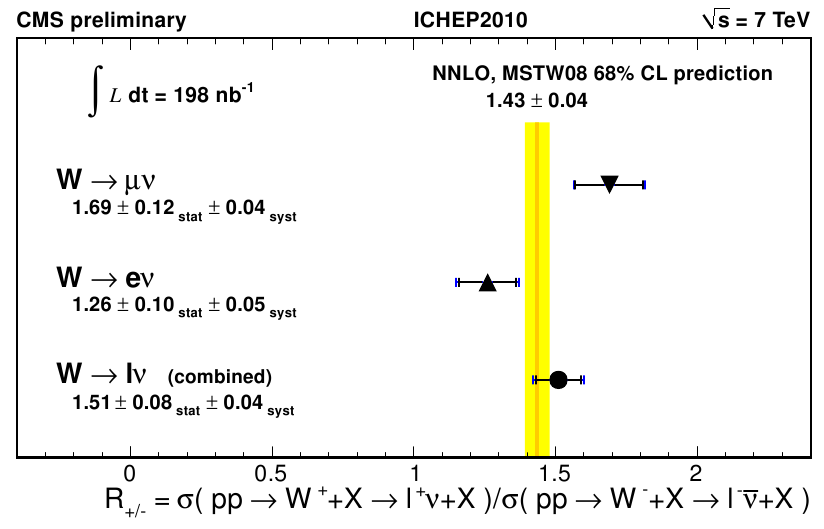
\includegraphics[width=0.95\linewidth]{Wcharge_ratio.png}

\end{center}
\column{0.58\linewidth}
\begin{center}
\textcolor{darkblue}{Number of jets produced with $W$}

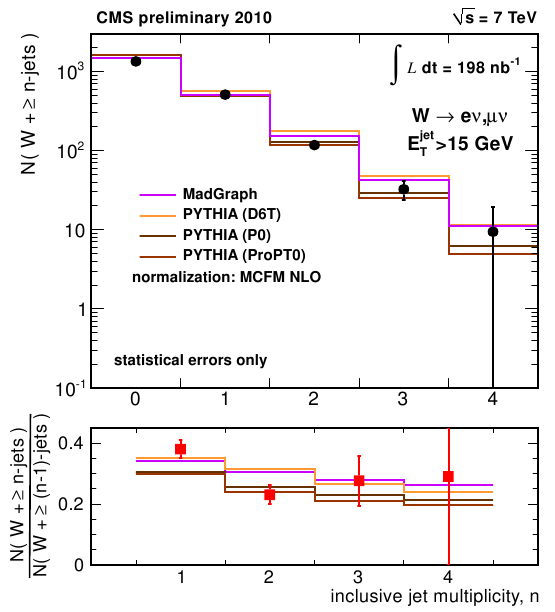
\includegraphics[width=\linewidth]{WplusJets.png}
\end{center}
\end{columns}
\end{frame}

\begin{frame}
\frametitle{Rediscovering the Standard Model}
\framesubtitle{The top quark}
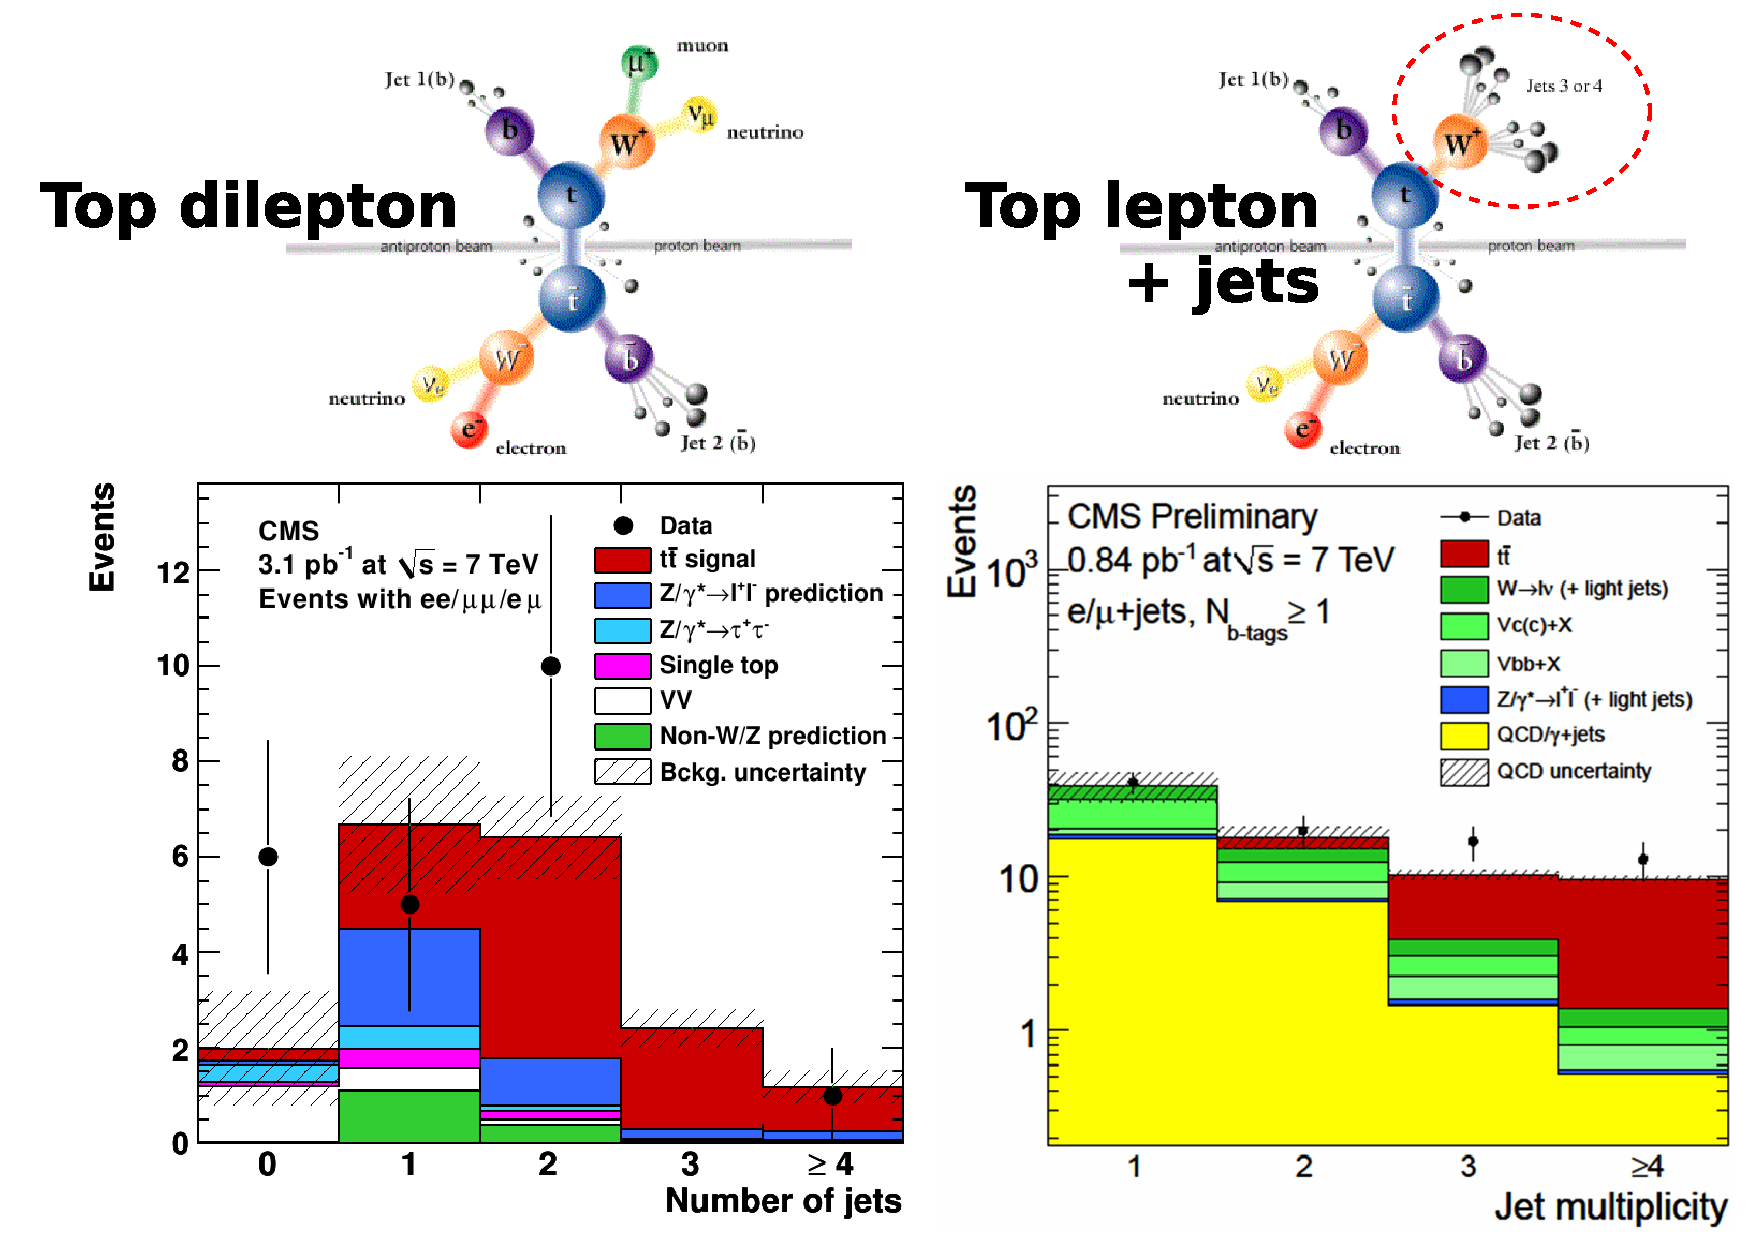
\includegraphics[width=\linewidth]{top.pdf}
\end{frame}

\begin{frame}
\frametitle{Rediscovering the Standard Model}
\framesubtitle{The top quark}
\begin{itemize}
\item Sample event display and mass in the dilepton channel
\item Lepton $p_T > 20$~GeV/$c$, relative isolation $<$ 15\% ($\Delta R < 0.3$), \\ $\not\!\!{E_{T}}$ $>$ 30~GeV (20~GeV for $e\mu$), $|M_{\ell\ell} - M_Z| > 15$~GeV/$c^2$
\end{itemize}
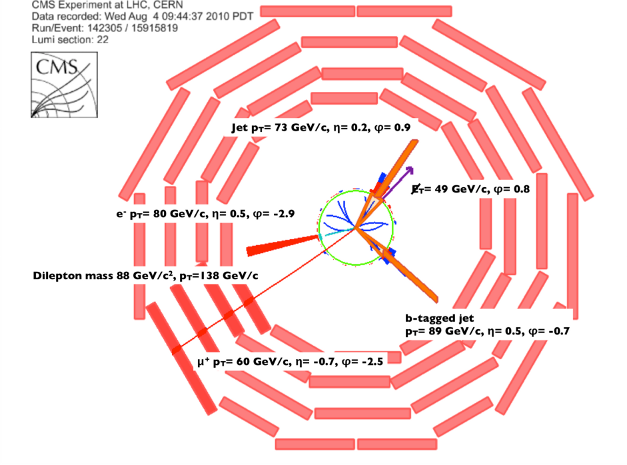
\includegraphics[width=0.55\linewidth]{top_e-mu_event.png}
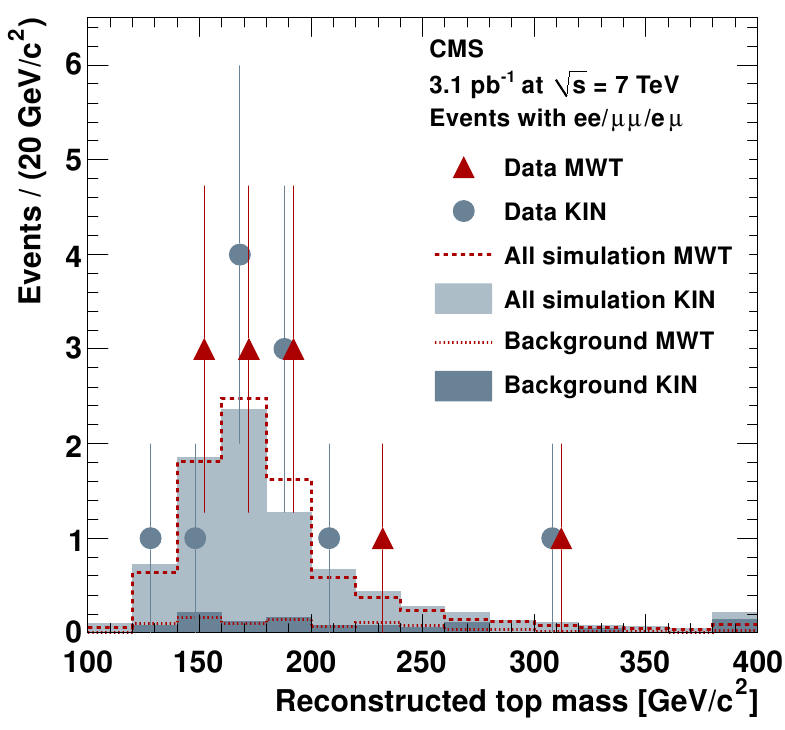
\includegraphics[width=0.45\linewidth]{newtop_mass.png}
\begin{itemize}
\item $\sigma(7\mbox{ TeV }pp \to t\bar{t})$ = 194 $\pm$ 72 (stat) $\pm$ 24 (syst) $\pm$ 21 (lumi) pb
\item NLO prediction: 157.5$^{+23.2}_{-24.4}$~pb \hfill (hep-ex/1010.5994)
\end{itemize}
\end{frame}

\begin{frame}
\frametitle{\underline{\bf Discovering} the Standard Model}
\begin{itemize}
\item Higgs discovery/limit-setting begins at 1~fb$^{-1}$, but can
  cover from the LEP limit (114~GeV/$c^2$) up to 600~GeV/$c^2$ with
  5~fb$^{-1}$, 8~TeV
\end{itemize}

\mbox{\hspace{-1.3 cm} \only<1>{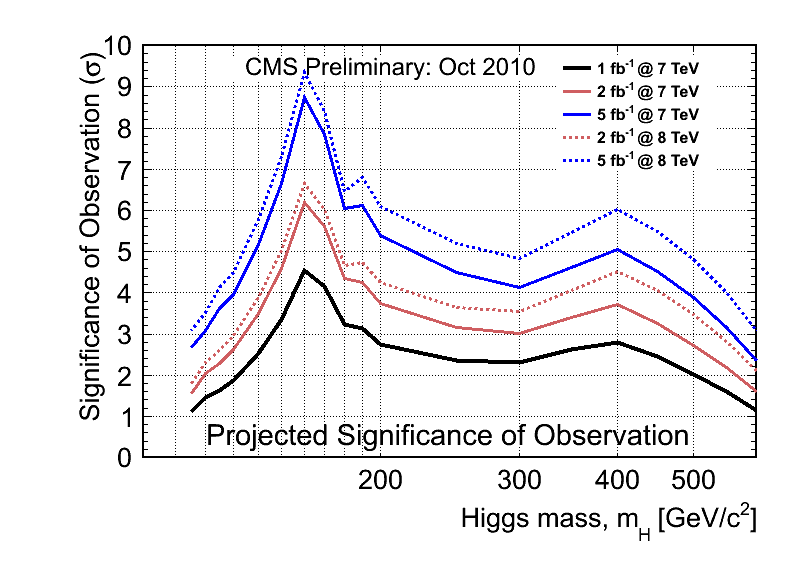
\includegraphics[width=0.6\linewidth]{newhiggs_observation.png}
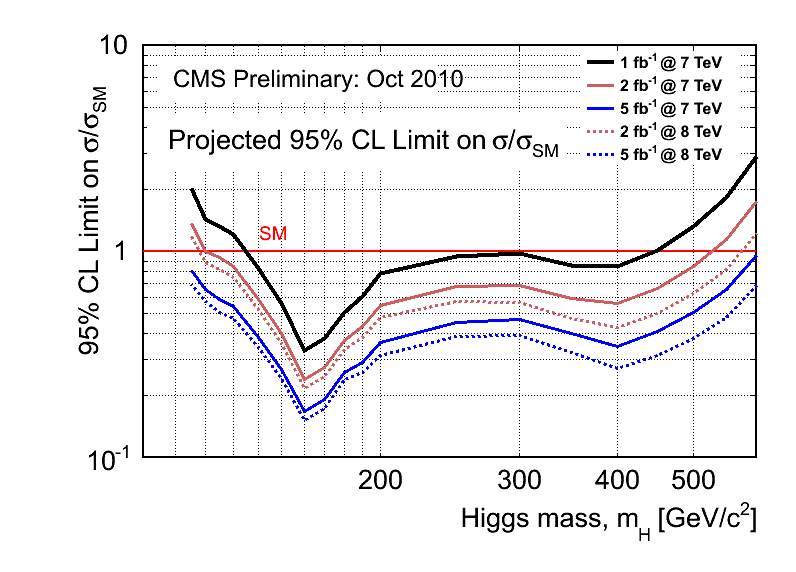
\includegraphics[width=0.6\linewidth]{newhiggs_limits.png}}\only<2>{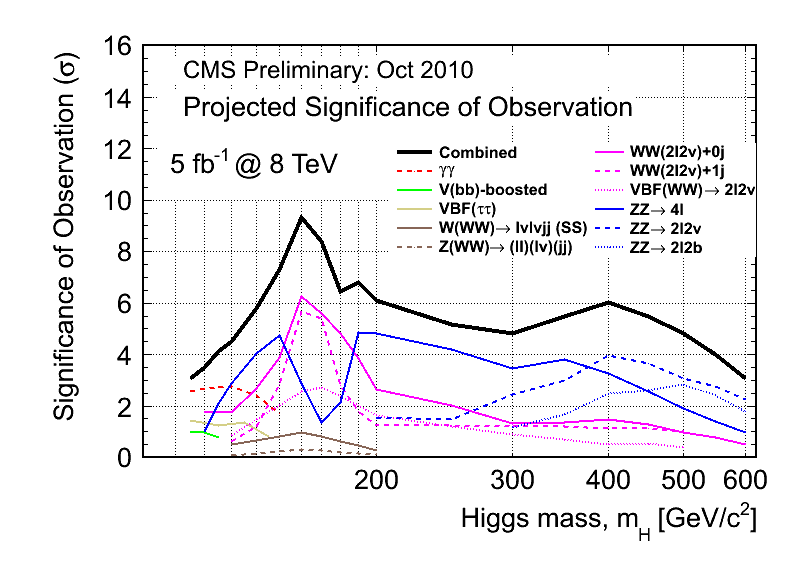
\includegraphics[width=0.6\linewidth]{newhiggs_observation_bymode.png}
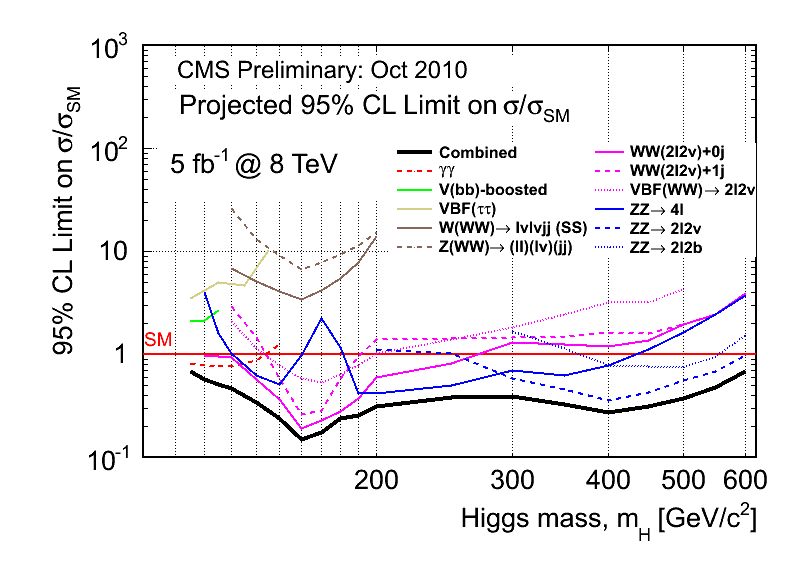
\includegraphics[width=0.6\linewidth]{newhiggs_limit_bymode.png}}}

\vspace{-0.3 cm}
\begin{itemize}
\item With 1~fb$^{-1}$, 7~TeV, ``ATLAS + CMS'' ($2\times$ CMS)
  projected $3\sigma$ sensitivity for $135 < m_H < 475$~GeV/$c^2$
\end{itemize}
\end{frame}

\section*{Beyond the Standard Model}
\begin{frame}
\begin{center}
\Huge \textcolor{blue}{Beyond the Standard Model}
\end{center}
\end{frame}

\begin{frame}
\frametitle{Beyond the Standared Model}
\framesubtitle{Dijet spectrum}
\begin{itemize}
\item Standard Model predicts a {\it smooth} distribution of dijet
  masses, new physics can produce narrow resonances: search for peaks

\item Anti-$k_T$ jets with $R=0.7$, both within $|\eta| < 2.5$, $|\Delta\eta| < 1.3$
\end{itemize}

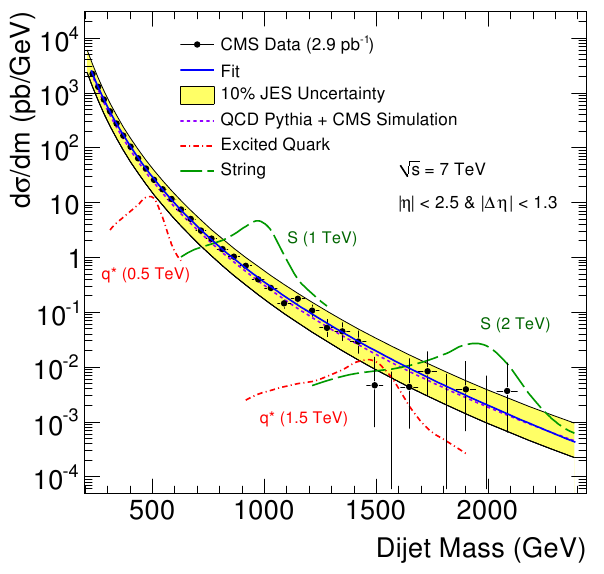
\includegraphics[height=5.3 cm]{dijet_spectrum.png} \hfill
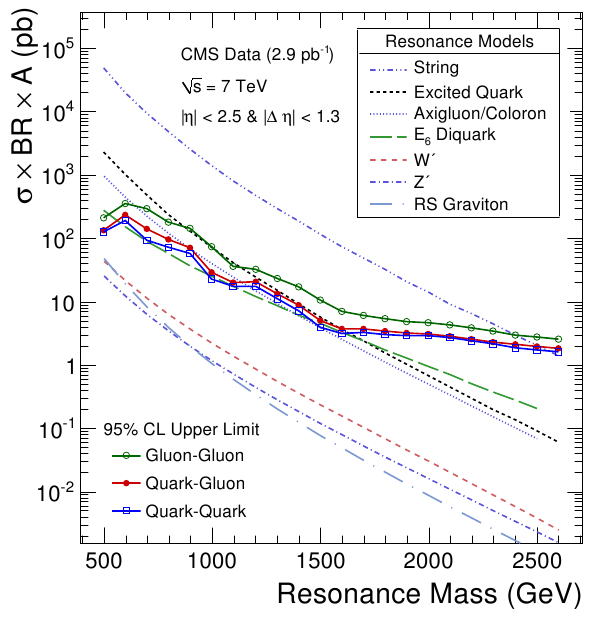
\includegraphics[height=5.3 cm]{dijet_limits.png}

\begin{itemize}
\item Extends previous limits; accepted by PRL (hep-ex/1010.0203)
\end{itemize}
\end{frame}

\begin{frame}
\frametitle{Beyond the Standared Model}
\framesubtitle{Dijet angular distributions}
\begin{columns}
\column{0.49\linewidth}
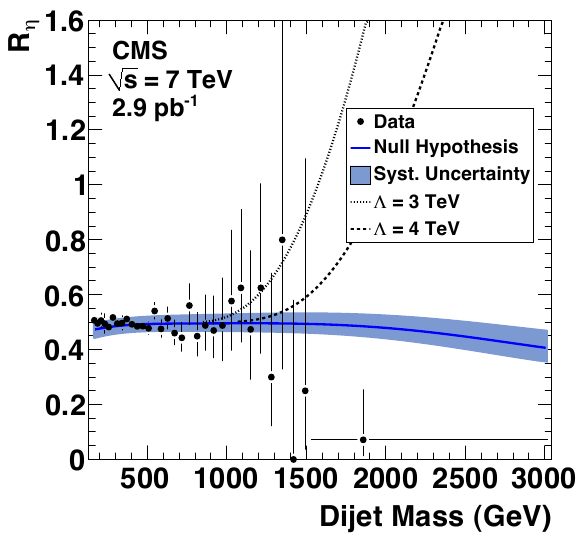
\includegraphics[width=\linewidth]{dijet_centrality_ratio.png}

\vspace{0.5 cm}
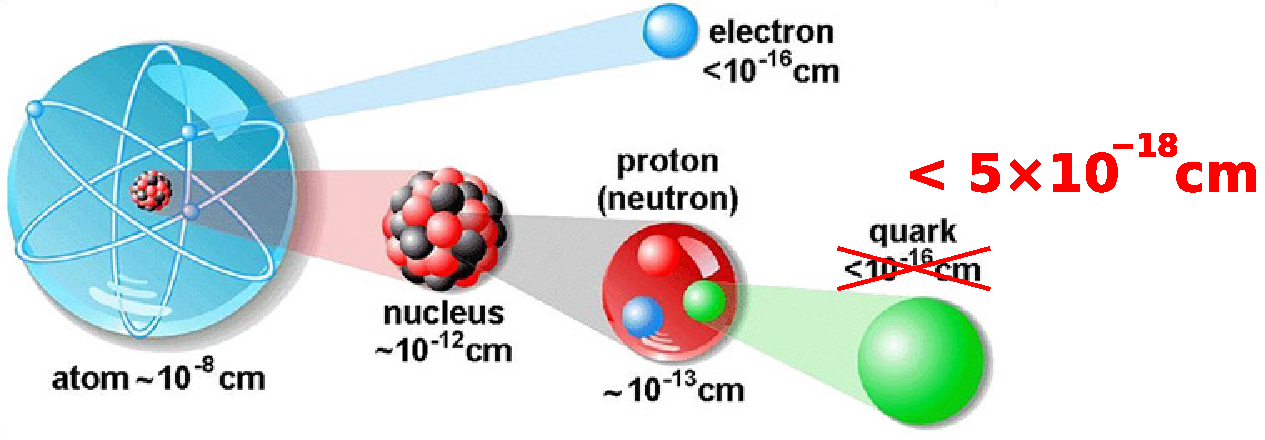
\includegraphics[width=\linewidth]{atom_zoom_b.pdf}

\column{0.5\linewidth}
\vspace{-0.3 cm}
\begin{itemize}
\item Standard Model jets are primarily at high $|\eta|$, new physics
  may be more central

\item Define centrality ratio

\mbox{$\displaystyle R_\eta = \frac{N_{jj}(|\eta| < 0.7)}{N_{jj}(0.7 < |\eta| < 1.3)}$}

where $N_{jj}(\cdot)$ is the number of events with both leading jets
in the specified range

\item Contact interaction $\Lambda < 4.0$~TeV at 95\% C.L. where effective Lagrangian

$\displaystyle \mathcal{L}_\s{eff} = \frac{2\pi}{\Lambda^2}
(\bar{q}_L \gamma^\mu q_L)(\bar{q}_L \gamma^\mu q_L)$

\item Extends limits; submitted to PRL (hep-ex/1010.4439)
\end{itemize}
\end{columns}
\end{frame}

\begin{frame}
\frametitle{Beyond the Standared Model}
\framesubtitle{Stopped $R$-hadrons}
\begin{columns}
\column{0.6\linewidth}
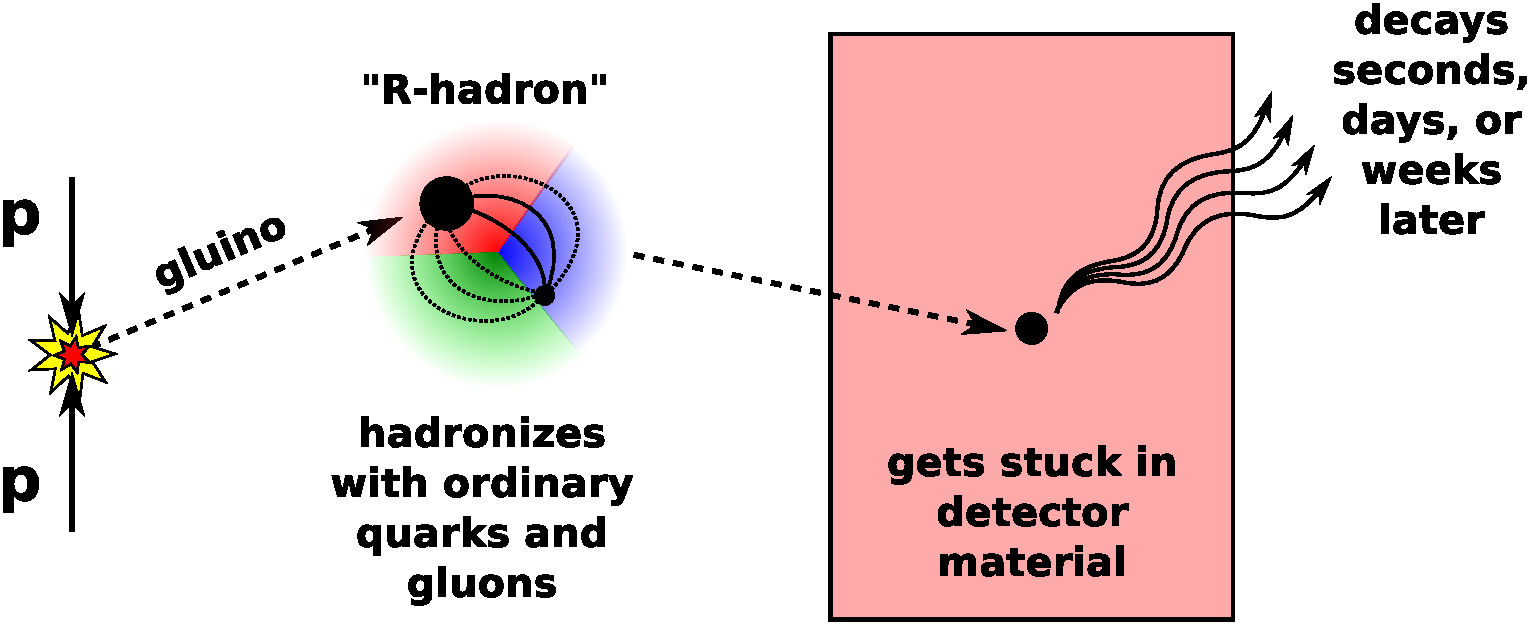
\includegraphics[width=\linewidth]{stoppedgluino.pdf}

\vspace{0.5 cm}
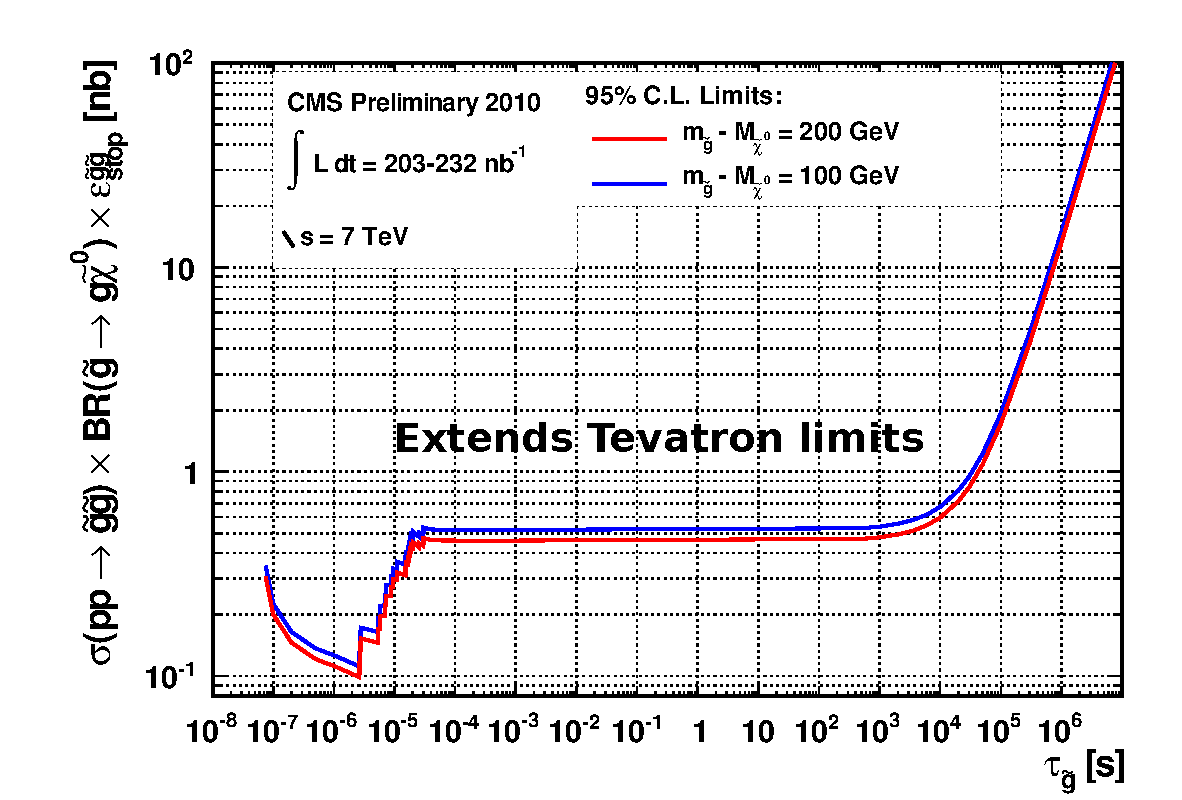
\includegraphics[width=\linewidth]{stoppedgluino_limits.pdf}

\column{0.5\linewidth}
\vspace{-0.25 cm}
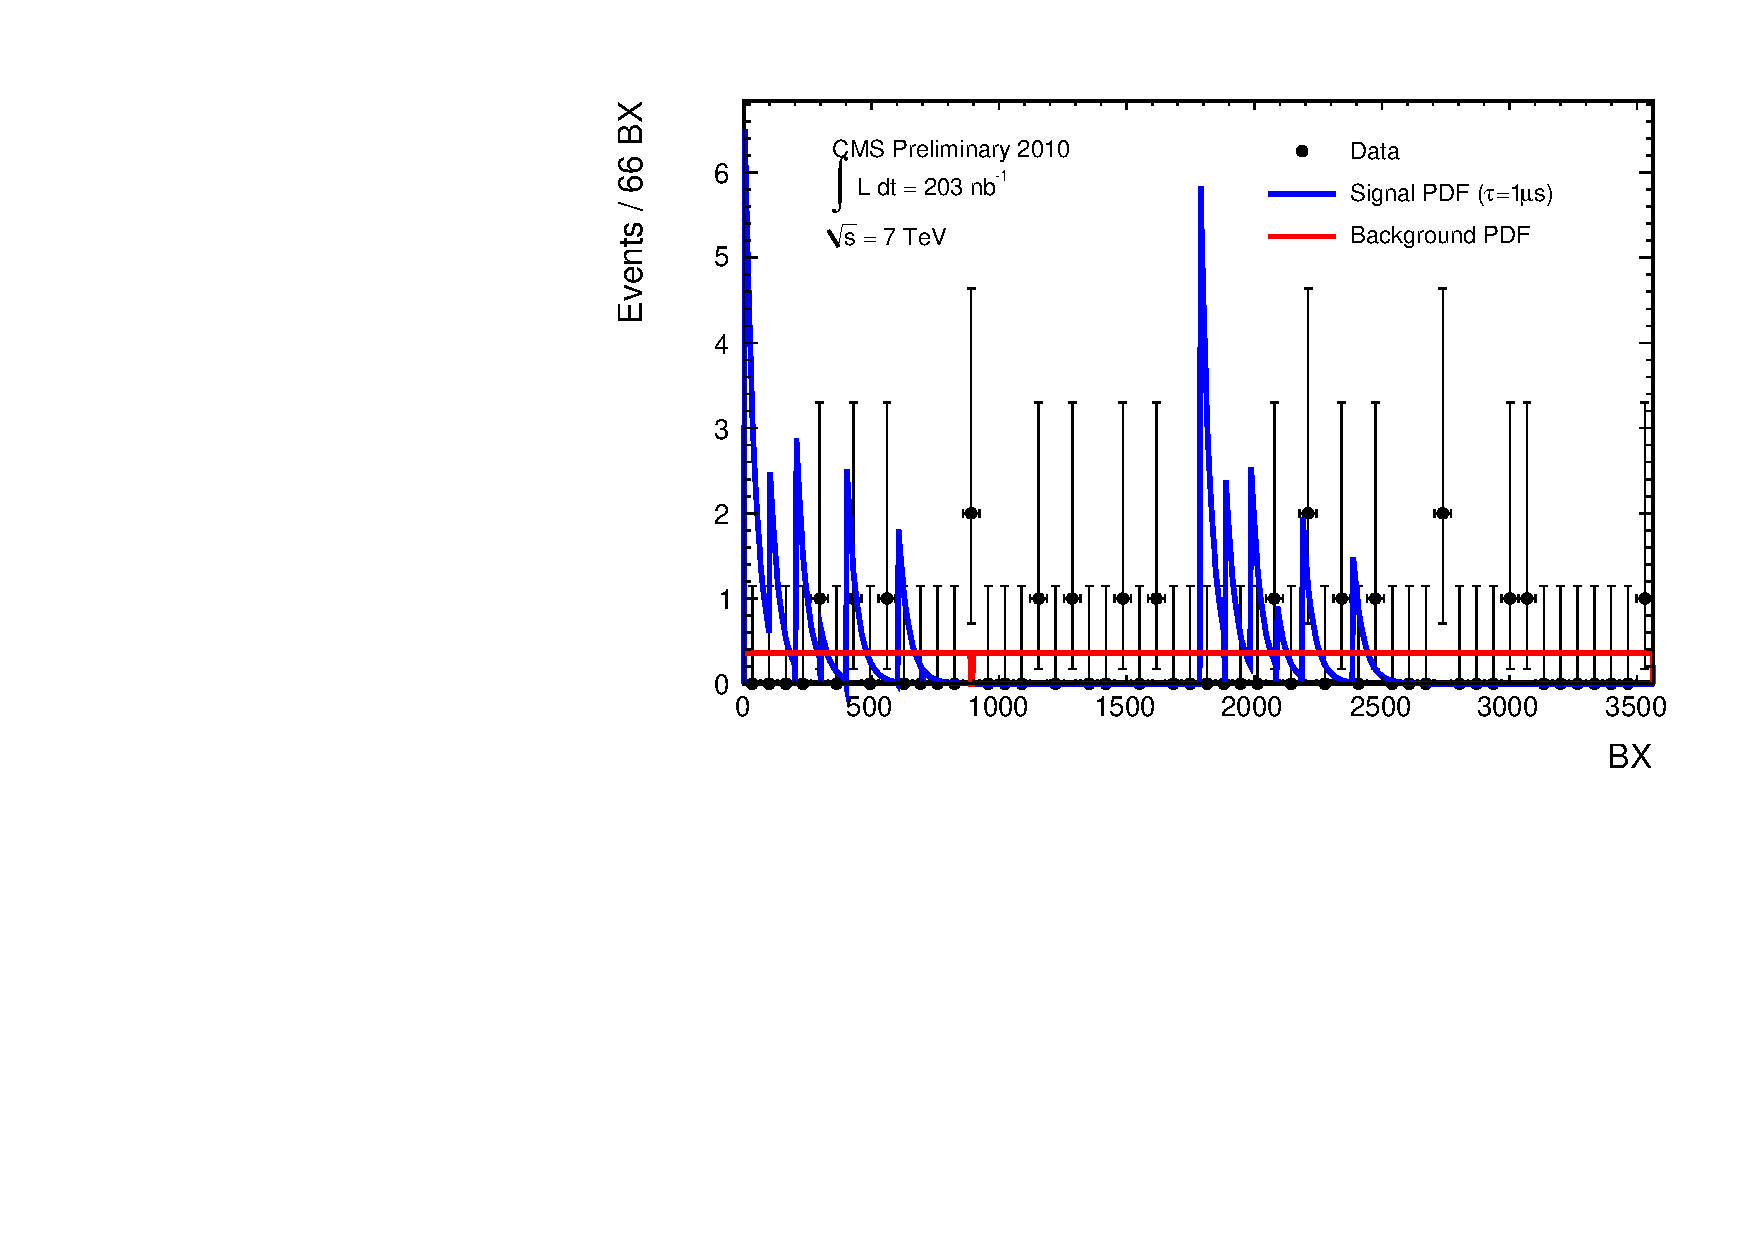
\includegraphics[width=\linewidth]{stoppedgluino_observedevents.pdf}

\begin{itemize}
\item 19 events observed in 115 hours of LHC operation (above) are
  consistent with expected backgrounds

\item Model-independent limits over 14 orders of magnitude in gluino
  lifetime (left)

\item $m_{\tilde{g}} <$ 229 (225) GeV/$c^2$ with a lifetime of 200~ns
  (2.6~$\mu$s) excluded
\end{itemize}
\end{columns}
\end{frame}

\begin{frame}
\frametitle{Beyond the Standared Model}
\framesubtitle{Other exotica results}
\begin{itemize}\setlength{\itemsep}{0.3 cm}
\item \textcolor{darkblue}{Heavy, stable charged particles:} identify
  tracks belonging to new, slow-moving ($\beta \lesssim 1$) particles
  by their energy loss ($dE/dx$)
\begin{itemize}
\item observed 0 events with 0.1 expected background (0.198~pb$^{-1}$)
\end{itemize}

\item \textcolor{darkblue}{Leptoquarks:} search for pairs of particles
  carrying both lepton number and baryon number: $\overline{\mbox{LQ}}\,\mbox{LQ} \to e\bar{q}\,eq$
\begin{itemize}
\item see Dinko Ferencek's talk
\end{itemize}

\item \textcolor{darkblue}{Extra dimensions from $G^* \to
  \gamma\gamma$:} spin-2 graviton can decay into two spin-1 bosons;
  clean signature
\begin{itemize}
\item see Duong Hai Nguyen's talk
\end{itemize}

\item Many others in progress
\end{itemize}
\end{frame}

\begin{frame}
\frametitle{Beyond the Standared Model}
\framesubtitle{Supersymmetry}

\mbox{\hspace{8.8 cm} \begin{minipage}{0.25\linewidth}
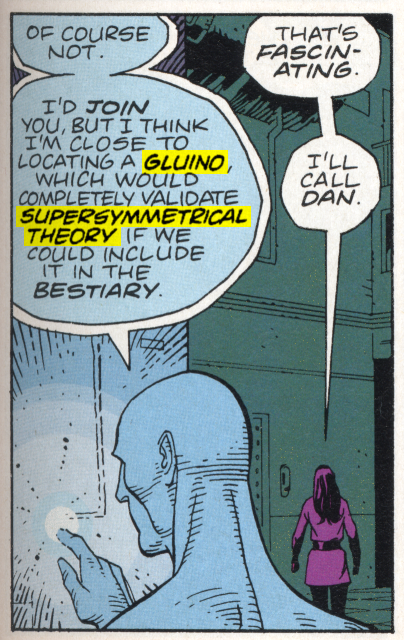
\includegraphics[width=\linewidth]{supersymmetrical_watchmen.png}

\centering {\it Watchmen,} 1987
\end{minipage}}

\vspace{-5 cm}
\begin{itemize}\setlength{\itemsep}{0.1 cm}
\item Many different signal topologies, all requiring \\
  100~pb$^{-1}$ or more

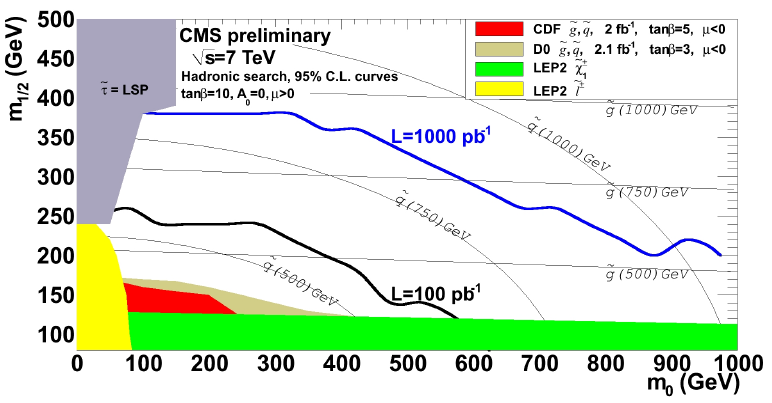
\includegraphics[width=0.75\linewidth]{susy_reach.png}

\item Developing a toolbox of techniques and studying QCD backgrounds
  with existing data
\begin{itemize}
\item high-$\not\!\!{E_{T}}$ tail, isolation, muons from decays in flight\ldots
\item verifying discriminating power of kinematic variables
\end{itemize}
\end{itemize}
\end{frame}

\begin{frame}
\frametitle{Beyond the Standared Model}
\framesubtitle{Supersymmetry example}

\begin{columns}
\column{0.47\linewidth}
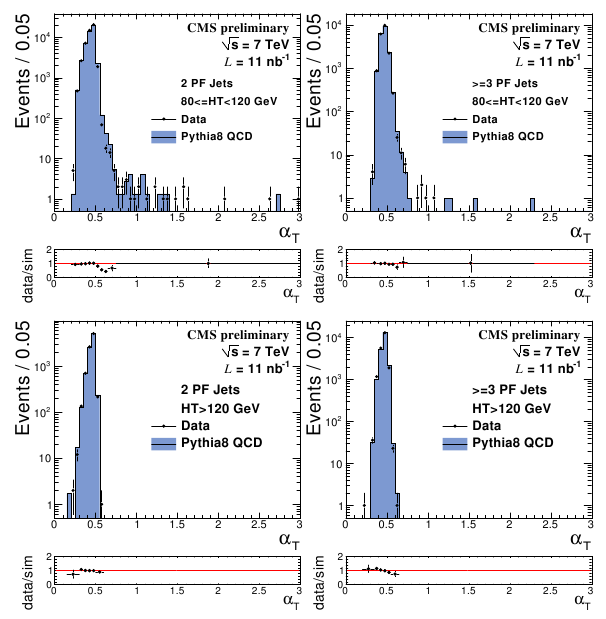
\includegraphics[width=\linewidth]{susy_example.png}
\column{0.6\linewidth}
\begin{itemize}
\item Data/MC comparison of $\alpha_T = p_{T2}/M_T$ where $p_{T2}$ is the second-highest jet momentum (with an extension to $N$-jets)

\item Complementary to $\displaystyle H_T = \sum_i^\s{jets} p_{Tj}$

\item Strong (4 orders of magnitude) supression of backgrounds in $\alpha_T > 0.55$ region
\end{itemize}
\end{columns}

\vspace{-0.3 cm}
\begin{tabular}{p{\linewidth}}
\\\hline
\end{tabular}

\vspace{0.2 cm}
\begin{columns}
\column{0.47\linewidth}
\includegraphics[width=\linewidth]{susy_mc.png}
\column{0.6\linewidth}
\begin{itemize}
\item MC study from a different paper, different cuts {\scriptsize ($H_T > 350$~GeV/$c$; tighter)}
\item Typical SUSY signals dominate in $\alpha_T > 0.55$ region
\end{itemize}
\end{columns}
\end{frame}

\section*{Expect the unexpected}
\begin{frame}
\begin{center}
\Huge \textcolor{blue}{Expect the unexpected}
\end{center}
\end{frame}

\begin{frame}
\frametitle{QCD angular correlations}
\begin{itemize}
\item Unexpected {\it physical} effect observed in min-bias track correlations

\item Definition of the correlation function:
{\tiny
\[ R(\Delta\eta, \Delta\phi) = \left\langle (\langle N \rangle - 1) \left(\frac{S_N(\Delta\eta, \Delta\phi)}{B_N(\Delta\eta, \Delta\phi)} - 1\right) \right\rangle_{\mbox{\tiny bins}} \]
\[ S_N(\Delta\eta, \Delta\phi) = \frac{1}{N(N-1)} \frac{d^2 N^{\mbox{\tiny signal}}}{d\Delta\eta d\Delta\phi} \mbox{, } B_N(\Delta\eta, \Delta\phi) = \frac{1}{N^2} \frac{d^2 N^{\mbox{\tiny mixed}}}{d\Delta\eta d\Delta\phi} \]}

\item Interpretation of the major features:
\begin{center}
\includegraphics[width=0.8\linewidth]{angularcorrelations.pdf}
\end{center}
\end{itemize}
\end{frame}

\begin{frame}
\frametitle{QCD angular correlations}
\includegraphics[width=\linewidth]{angularcorrelations_four.pdf}
\end{frame}

\begin{frame}
\frametitle{QCD angular correlations}
\begin{itemize}
\item This structure resembles features observed in heavy ion experiments
\item \it But the physical origin of our observation is not yet understood
\end{itemize}

\vspace{-0.3 cm}
\begin{center}
\includegraphics[height=5 cm]{angularcorrelations_big.png}
\includegraphics[height=5 cm]{angularcorrelations_phobos.png}
\end{center}

\vspace{-0.3 cm}
\begin{itemize}
\item hep-ex/1009.4122
\end{itemize}
\end{frame}

\section*{The triumph of optimism}
\begin{frame}
\begin{center}
\Huge \textcolor{blue}{``The triumph of optimism''}
\end{center}
\end{frame}

\begin{frame}
\frametitle{The triumph of optimism}
\begin{itemize}
\item Conventional wisdom: ``be wary of techniques that rely on a
  detailed understanding of the detector until the experiment has
  become mature\ldots''  Things like
\begin{itemize}
\item material budget
\item alignment
\item $b$-tagging
\item particle flow
\item missing energy
\end{itemize}

\item But the start-up has been a lot smoother than anticipated, with
  many features well-described by simulation very early

\item<2> For example, material budget (as seen by $\gamma$-conversions):

\begin{center}
\includegraphics[height=3 cm]{material_conversions_r.png}
\includegraphics[height=3 cm]{material_conversions_eta.png}
\end{center}
\end{itemize}
\end{frame}

\begin{frame}
\frametitle{The triumph of optimism}
\begin{itemize}
\item Alignment had an extra year to improve with cosmics, so test the Cosmics Alignment with the primary vertex:
\begin{columns}
\column{0.3\linewidth}
\includegraphics[height=3 cm]{alignment_2.png}

\column{0.2\linewidth}
\scriptsize Fit the vertex with $N-1$ tracks, plot distance of closest approach of
the probe track

\column{0.4\linewidth}
\includegraphics[height=3 cm]{alignment_1.png}
\end{columns}

\item<2> \ldots which is useful for $b$-tagging:

\includegraphics[width=0.32\linewidth]{btag_3dsignificance.png}
\includegraphics[width=0.32\linewidth]{btag_muonpt.png}
\includegraphics[width=0.32\linewidth]{btag_discriminator.png}
\end{itemize}
\end{frame}

\begin{frame}
\frametitle{The triumph of optimism}
\begin{itemize}
\item Particle flow:

\includegraphics[height=3.3 cm]{particleflow_electronid.pdf}
\includegraphics[height=3.3 cm]{particleflow_met.png}

\item<2> \ldots which is useful for missing energy:

\includegraphics[height=3 cm]{met_calo.png}
\includegraphics[height=3 cm]{met_pf.png}
\includegraphics[height=3 cm]{met_pf_nongauss.pdf}
\end{itemize}
\end{frame}

\section*{Conclusions}
\begin{frame}
\frametitle{Conclusions}
\begin{itemize}
\item Expectations for the first year of LHC physics were not set too high:

\vspace{-0.2 cm}
\begin{itemize}\setlength{\itemsep}{0.2 cm}
\item CMS followed the rapid rise in LHC luminosity, having collected
  over 40~pb$^{-1}$ of quality data (and counting)
\item the Standard Model was rediscovered quickly; top quarks {\it do}
  exist in Europe
\item exotica searches that rely on high center-of-mass energy are
  already extending world limits
\item the feature in two-particle correlations was unexpected,
  perhaps the first taste of surprises yet to come
\end{itemize}

\item In many ways, the 2010 results and maturity of the detector
  exceeded even the most optimistic expectations for the first physics
  run of the LHC

\item Soon we will be entering the SUSY/Higgs-search era: looking
  forward to the resolution of 30 years of anticipation\ldots
\end{itemize}
\label{numpages}
\end{frame}

\end{document}
